\externaldocument{chap02}
\externaldocument{chap03}
\externaldocument{chap04}


\chapter{视觉惯性定位系统搭建与测试}

本章主要对定位系统的搭建即实施进行介绍。首先介绍了定位系统运行所依靠的硬件平台以及软件环境,不同于一般的定位系统,本文方法的实施依赖于深度学习及图形处理单元(Graphics processing unit, GPU)。然后介绍了本文所使用的数据集以及评价指标,本文实验主要建立在3个数据集上,分别是KITTI数据集、4Seasons数据集和KAIST数据集,其中KITTI数据集场景相对单一,适合验证离线建图模块的性能,以及初步验证定位模块的性能;4Seasons数据集提供的场景丰富,适合验证VIO和紧耦合地图定位模块的性能;KAIST数据集提供了超长轨迹,适合验证VIO模块的性能。最后本章介绍了定位系统三个模块的测试结果,并通过相应的消融实验来验证各部分的真实作用。

\section{系统与测试细节}
\subsection{硬件与软件环境}

本文所设计的定位系统的运行环境依赖于同时具有CPU(Central processing unit)和GPU(Graphics processing unit)的计算机,具体来说本文所实验的平台使用12th Gen Intel(R) Core(TM) i7-12700 CPU和NVIDIA GeForce RTX 3080 GPU。

\begin{figure}
  \centering
  \subcaptionbox*{Ubuntu 20.04 LTS}{
\includegraphics[width=0.22\linewidth]{ubuntu_logo.png}}
  \subcaptionbox*{ROS Noetic}{
\includegraphics[width=0.18\linewidth]{noetic_logo.png}}
  \subcaptionbox*{VINS-Mono}{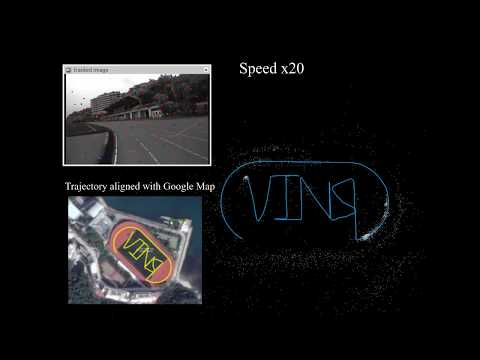
\includegraphics[width=0.22\linewidth]{VINS_logo.jpeg}}
  \subcaptionbox*{TensorRT}{
\includegraphics[width=0.3\linewidth]{tensorrt_logo.png}}
  \caption{软件部署环境}
  \label{fig:software}
\end{figure}

系统的软件部署环境如图~\ref{fig:software} 所示,其中Ubuntu 20.04 LTS是本文所使用的操作系统;ROS Noetic是本文所使用的机器人操作系统,其主要作用是将多个子系统的结果方便快捷地统一处理;VINS-Mono是本文所使用的视觉惯性定位系统的基线,其具有较为简洁的逻辑划分,方便快速改进、验证想法;TensorRT是本文所使用的深度学习推理框架,其主要负责系统中的神经网络推理任务,其针对NVIDIA显卡的速度优化使得整个系统可以实时运行。此外,本文所设计系统中还有大量超参数,其具体取值如表~\ref{tab:hyperparameters} 所示。

\begin{table}
\centering
\caption{本文中所涉及的运行超参数}
\begin{tabular}{lccc}
\toprule
参数名 & 首次出现章节 & 作用 & 取值 \\
\midrule
$t_l$ & \ref{sec:map_sfm} & SfM中回环检测相似度阈值 & 0.8 \\
$m$ & \ref{sec:map_sfm} & SfM中回环帧数量 & 5 \\
$\alpha$ &  \ref{sec:map_fusion}  & 建图融合权重系数     & 1000 \\
$\tau$ & \ref{sec:network_design} & 车辆状态正例预测阈值 & 0.9 \\
$N_c$ & \ref{sec:loc_vote}  & 粗到细匹配候选关键帧数量 & 7   \\
$t_r$ &  \ref{sec:loc_vote}  & 投票过程相对旋转角度阈值 & $15\degree$   \\
$t_p$ &  \ref{sec:loc_vote}  & 投票过程相对位移阈值   & 5m    \\
$\lambda_r$ &  \ref{sec:valid}  & 有效性验证角度阈值    & $60\degree$   \\
$\lambda_p$ &  \ref{sec:valid}  & 有效性验证位移阈值    & 15m   \\
$N$ &  \ref{sec:loc_pg}  & 滑动窗口容量       & 20   \\
$\kappa$ &  \ref{sec:loc_pg}  & 单帧图像所考虑的点云比例 & 10  \\
\bottomrule
\end{tabular}
\label{tab:hyperparameters}
\end{table}

\subsection{测试数据集与评价指标}
\subsubsection{KITTI数据集}
KITTI 数据集\cite{Geiger2012CVPR}是SLAM和自动驾驶研究中最受欢迎且使用广泛的数据集之一,它包含大量的多种传感器采集的交通场景数据,包括高分辨率RGB双目相机图像、灰度双目相机图像以及3D激光雷达数据。该数据集提供了11条经过精心选择的序列,构成视觉里程计基准。每条序列包含来自四个相机的数据:两个灰度相机和两个彩色相机。此外,KITTI 数据集还为这11条视觉里程计基准序列中的10条提供了原始GNSS观测数据和IMU测量数据。

\begin{figure}
  \centering
  \subcaptionbox*{序列00-城镇环境}{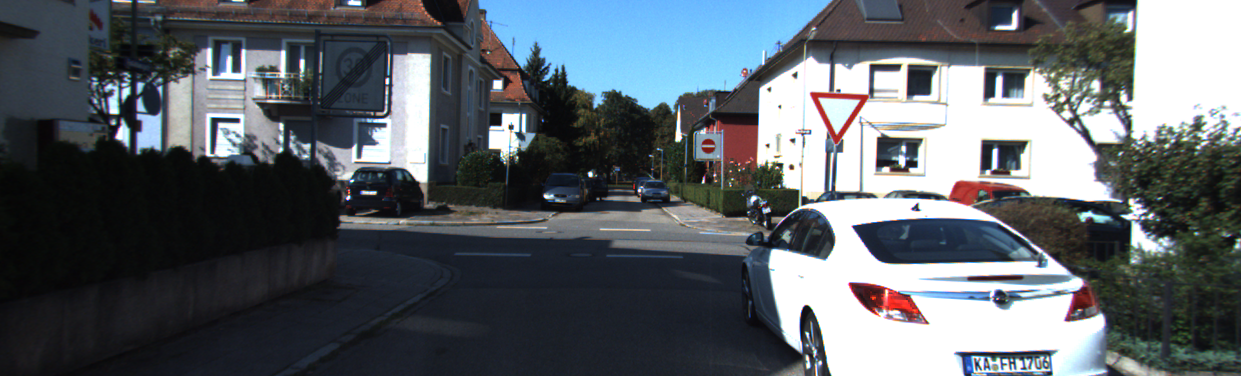
\includegraphics[width=0.47\linewidth]{kitti_00.png}}
  \subcaptionbox*{序列01-高架环境}{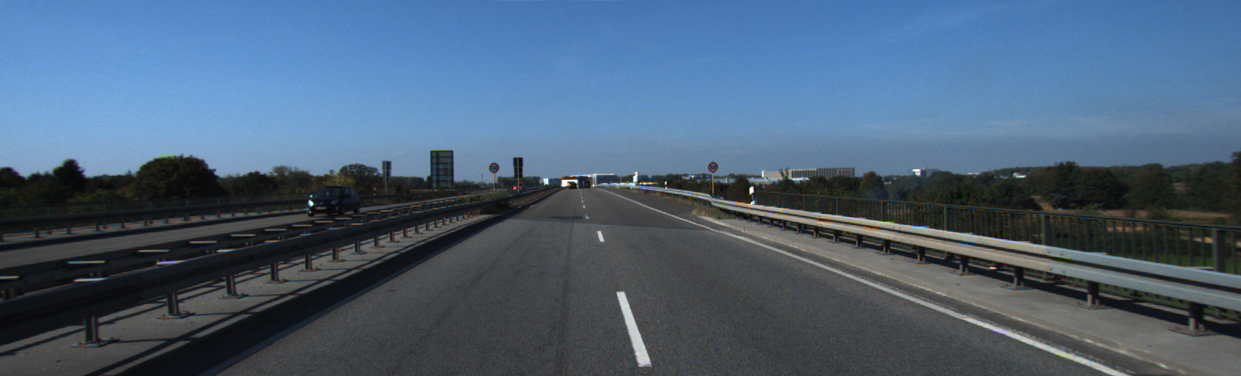
\includegraphics[width=0.47\linewidth]{kitti_01.png}}
  \subcaptionbox*{序列09-郊外环境}{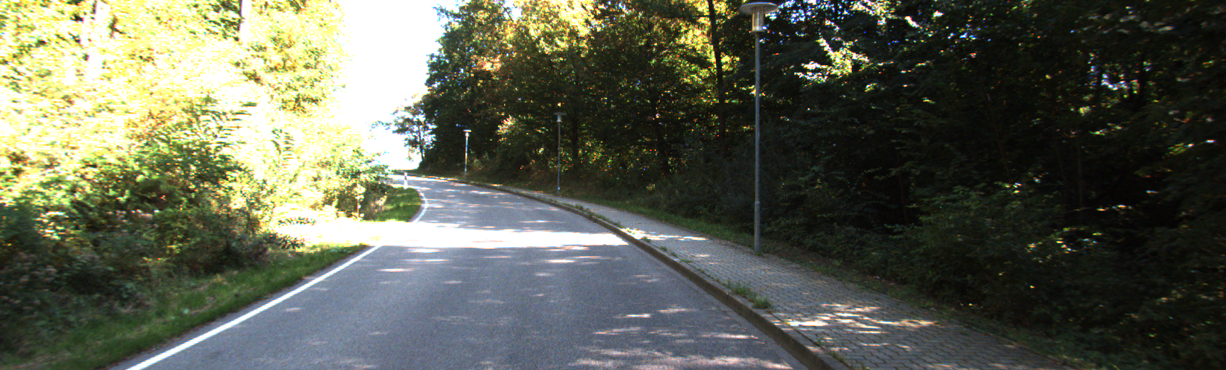
\includegraphics[width=0.47\linewidth]{kitti_09.png}}
  \subcaptionbox*{序列10-农村环境}{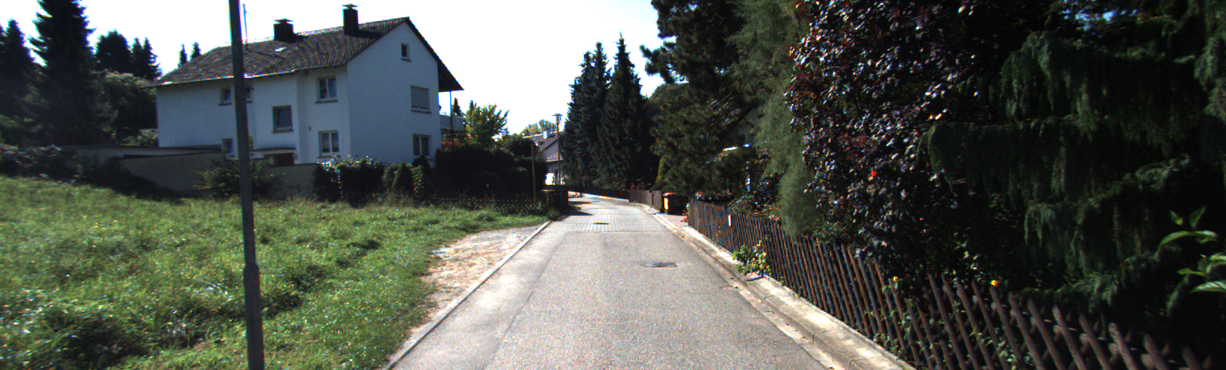
\includegraphics[width=0.47\linewidth]{kitti_10.png}}
  \caption{KITTI数据集场景}
  \label{fig:kitti_data}
\end{figure}

本文使用KITTI视觉里程计基准中包含GNSS观测数据的10条序列,评估本文所提出系统的建图性能以及整体性能。这10条序列包括了城镇、高架、郊外以及农村等常见的车辆行驶环境,如图~\ref{fig:kitti_data} 所示。

\subsubsection{4Seasons数据集}
4Seasons数据集\cite{wenzel20214seasons}是一个专为自动驾驶研究设计的数据集,提供了涵盖季节变化和复杂感知条件的图像、IMU等数据。同一路径在不同季节和多种感知条件下被多次采集,使其特别适合于评估针对固定路径设计的方法。该数据集使用的传感器包括立体相机、IMU和RTK-GNSS,同时还提供了精度达到厘米级的高精度真值位姿。

与KITTI数据集相比,4Seasons数据集能够提供更具挑战性和说服力的实验结果,突出了本文方法的优势。本文选择了四个具有代表性的场景,分别是

\textbf{(1)Office Loop (OF):} 位于城郊工业区的环形路线,长度约为3776米,包含了多种感知条件,如建筑物、树木和道路标志等,如图~\ref{fig:OF_data} 所示。此路线在不同季节采集了5条序列(以OF1-5代称),每条序列包含了来自灰度立体相机、IMU和RTK-GNSS的数据。
\begin{figure}
  \centering
  \subcaptionbox*{场景感知条件}{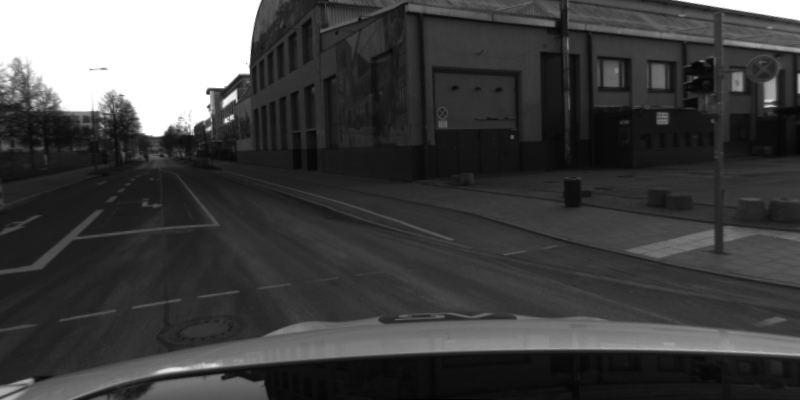
\includegraphics[width=0.48\linewidth]{OfficeLoop.png}}
  \subcaptionbox*{路径卫星图}{\includegraphics[width=0.48\linewidth]{gnss_OF1.png}}
  \caption{Office Loop场景}
  \label{fig:OF_data}
\end{figure}

\textbf{(2) Neighborhood (NH):} 位于城镇环境的环形路线,长度约为2106米,包含了多种感知条件,如树木和房屋等,包含了更多的植被,接近于农村环境,如图~\ref{fig:NH_data} 所示。此路线在不同季节采集了7条序列(以NH1-7代称),每条序列包含了来自灰度立体相机、IMU和RTK-GNSS的数据。

\begin{figure}
  \centering
  \subcaptionbox*{场景感知条件}{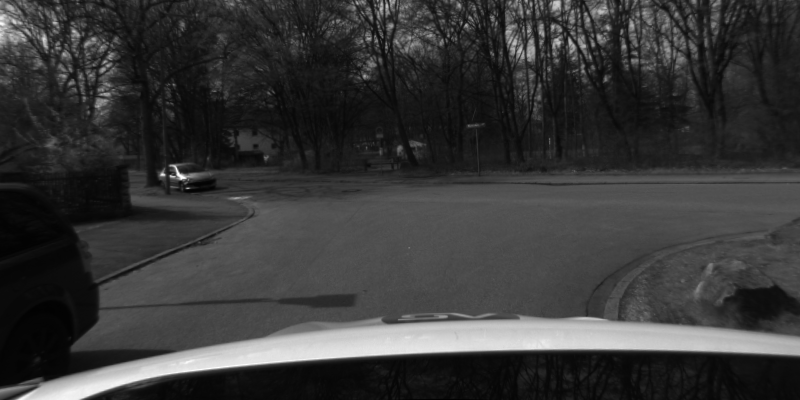
\includegraphics[width=0.48\linewidth]{Neighborhood.png}}
  \subcaptionbox*{路径卫星图}{\includegraphics[width=0.48\linewidth]{gnss_NH01.png}}
  \caption{Neighborhood场景}
  \label{fig:NH_data}
\end{figure}

\textbf{(3) Business Campus (BC):} 位于校园和商业区的多条环形路线,长度约为3011米,包含了更多的建筑物,如图~\ref{fig:BC_data} 所示。此路线在不同季节采集了3条序列(以BC1-3代称),每条序列包含了来自灰度立体相机、IMU和RTK-GNSS的数据。

\begin{figure}
  \centering
  \subcaptionbox*{场景感知条件}{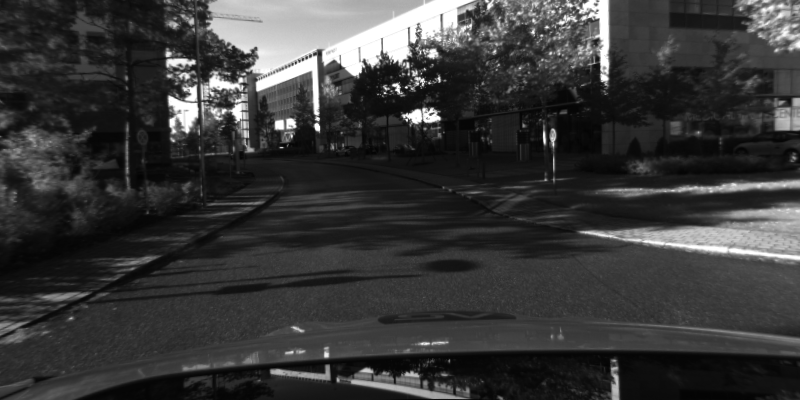
\includegraphics[width=0.48\linewidth]{BusinessCampus.png}}
  \subcaptionbox*{路径卫星图}{\includegraphics[width=0.48\linewidth]{gnss_BC1.png}}
  \caption{Business Campus场景}
  \label{fig:BC_data}
\end{figure}

\textbf{(4) Old Town (OT):} 位于城市中心的商业区环线,长度约为5034米,包含了多种感知条件,此外还有大量的移动物体,如汽车、行人和自行车等,如图~\ref{fig:OT_data} 所示。此路线在不同季节采集了2条序列(以OT1-3代称),每条序列包含了来自灰度立体相机、IMU和RTK-GNSS的数据。

\begin{figure}
  \centering
  \subcaptionbox*{场景感知条件}{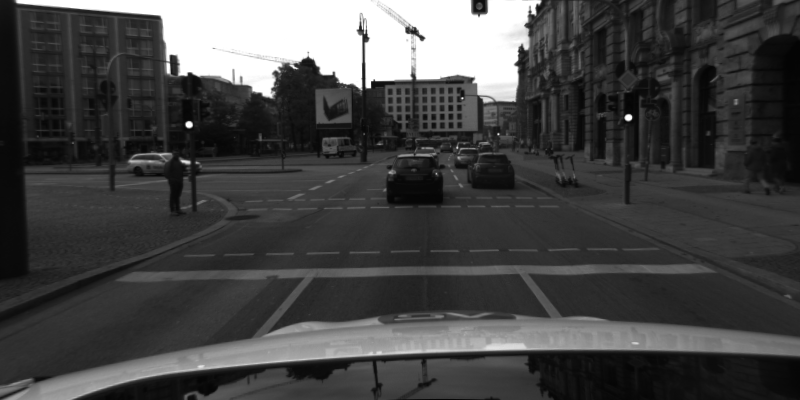
\includegraphics[width=0.48\linewidth]{OldTown.png}}
  \subcaptionbox*{路径卫星图}{\includegraphics[width=0.48\linewidth]{gnss_OT1.png}}
  \caption{Old Town场景}
  \label{fig:OT_data}
\end{figure}

\subsubsection{KAIST数据集}
KAIST数据集\cite{jjeong-2019-ijrr}同时提供了LiDAR(Light Detection And Ranging)、立体相机、GPS、IMU、编码器和气压计等多种传感器数据,使得用户可以针对不同传感器组合进行多模态信息处理。采集环境涵盖了从多车道宽阔道路到高密度城市街区等多种复杂场景,这不仅体现了实际城市环境中GPS信号不稳定、遮挡严重等问题,也为算法在动态、遮挡等极端条件下的鲁棒性验证提供了真实数据。此外,数据集通过高精度传感器与消费者级传感器的双层数据采集,以及精细的时间同步和标定处理,确保了数据的高准确性和一致性,并提供了基准轨迹及ROS工具,极大地方便了机器人定位、SLAM及环境感知等相关领域的研究与测试。

本文中主要选择了KAIST数据集中的三个场景,分别是20-Highway、26-Dongtan和28-Pangyo,如图~\ref{fig:KAIST_data} 所示。这三个场景分别代表了高速公路、郊区和城市环境,适合于测试本文方法在不同场景下的性能。其中28-Pangyo是一段超过10公里的城市环境,包含了大量的建筑物、行人和车辆,是一个非常具有挑战性的场景。KAIST数据集主要被使用来评估本文的VIO模块性能。

\begin{figure}
  \centering
  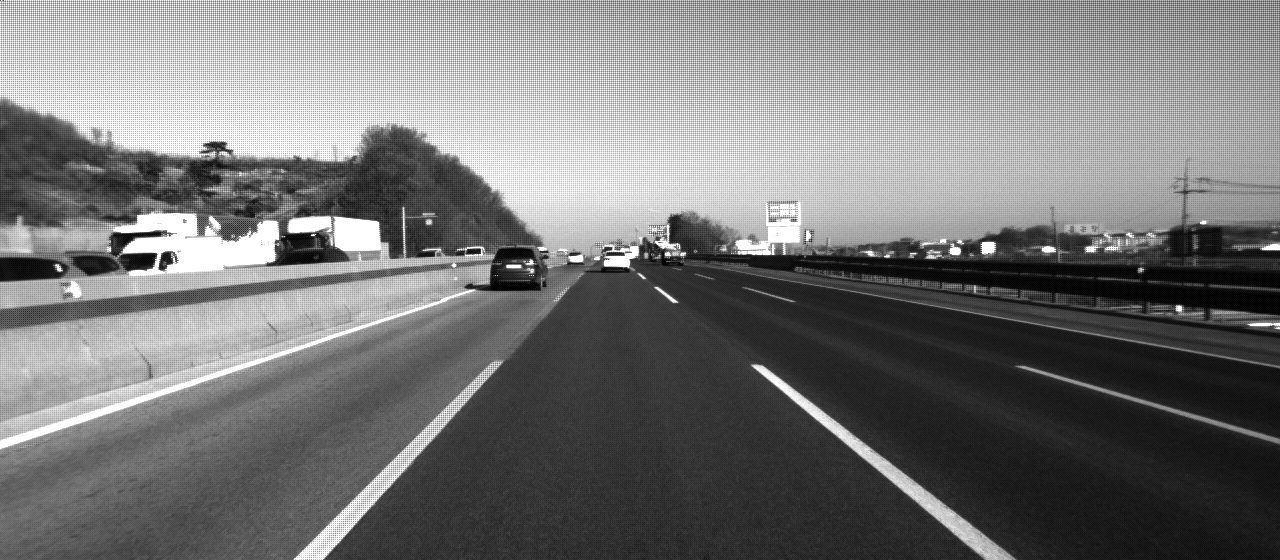
\includegraphics[width=0.32\linewidth]{KAIST_20_scene.png}
  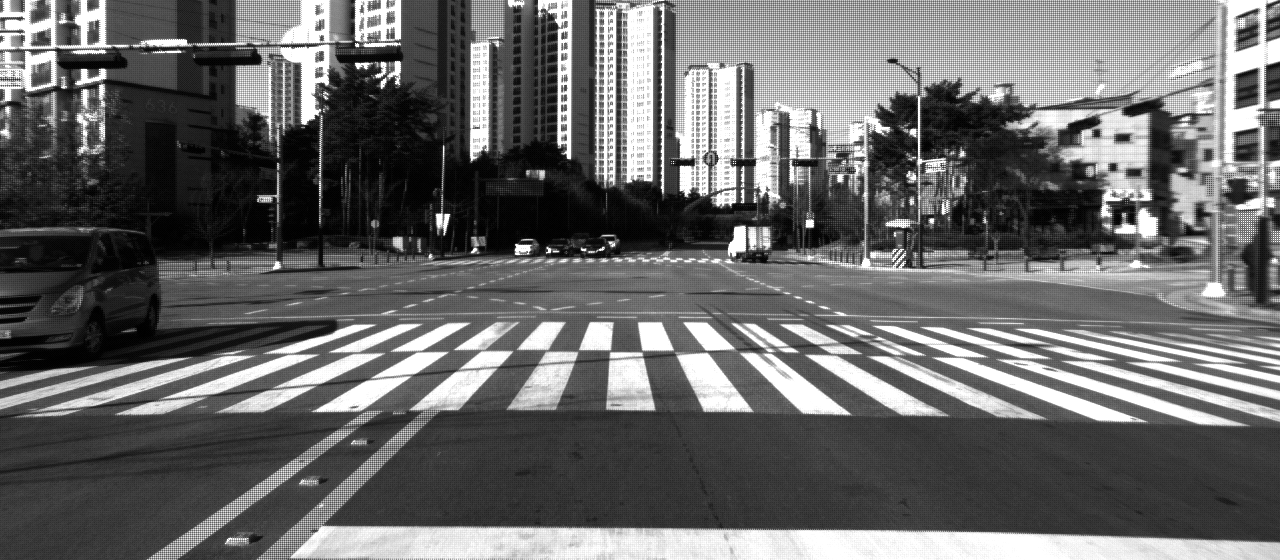
\includegraphics[width=0.32\linewidth]{KAIST_26_scene.png}
  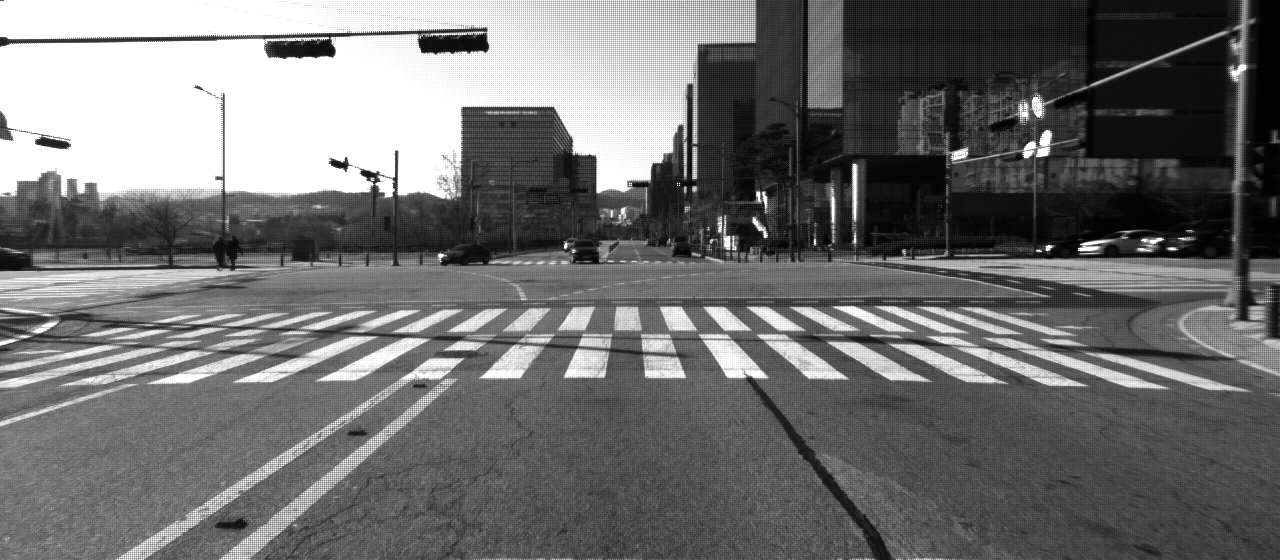
\includegraphics[width=0.32\linewidth]{KAIST_28_scene.png}
  \subcaptionbox*{序列20-Highway}{\includegraphics[width=0.32\linewidth]{KAIST_20.png}}
  \subcaptionbox*{序列20-Dongtan}{\includegraphics[width=0.32\linewidth]{KAIST_26.png}}
  \subcaptionbox*{序列20-Pangyo}{\includegraphics[width=0.32\linewidth]{KAIST_28.png}}
  \caption{KAIST数据集场景}
  \label{fig:KAIST_data}
\end{figure}

\subsubsection{数据集使用划分}

由于本文需要分别验证3个模块的效果,因此本文将数据集的划分总结如表~\ref{tab:dataset_usage} 所示。表中的每一列代表了一个测试模块,每一行代表了一个数据集,表中的符号代表了数据集的使用方法,其中{\color[HTML]{3166FF} $\bigcirc$}代表使用该序列进行训练或者建图,{\color[HTML]{FD6864}$\bigtriangleup$}代表使用该序列进行测试。

\begin{table}
\centering
\begin{threeparttable}
\caption{数据集使用划分}
\begin{tabular}{lccccccc}
\toprule
\multirow{2}{*}{测试模块} & \multicolumn{2}{c}{KITTI}               & \multicolumn{4}{c}{4Seasons}   & KAIST                                         \\ \cline{2-8} 
                  & 灰色                          & 彩色         & OF1              & OF2-5            & \begin{tabular}[c]{@{}c@{}}NH1 \\ BC1 \\ OT1\end{tabular} & \begin{tabular}[c]{@{}c@{}}NH2-7 \\ BC2-3 \\ OT2-3\end{tabular} & \begin{tabular}[c]{@{}c@{}}20-Highway  \\ 26-Dongtan \\ 28-Pangyo\end{tabular} \\ \midrule
离线建图模块 & {\color[HTML]{3166FF} $\bigcirc$}{\color[HTML]{FD6864}$\bigtriangleup$} &            &                  &                  &               &         &          \\
PO-VIO模块           &                             &            & {\color[HTML]{FD6864}$\bigtriangleup$} & {\color[HTML]{FD6864}$\bigtriangleup$} & {\color[HTML]{3166FF} $\bigcirc$}    &         &     {\color[HTML]{FD6864}$\bigtriangleup$}     \\
地图定位模块           & {\color[HTML]{FD6864}$\bigtriangleup$}           & {\color[HTML]{3166FF} $\bigcirc$} & {\color[HTML]{3166FF} $\bigcirc$}       & {\color[HTML]{FD6864}$\bigtriangleup$} & {\color[HTML]{3166FF} $\bigcirc$}    & {\color[HTML]{FD6864}$\bigtriangleup$} & \\ \bottomrule
\end{tabular}
\label{tab:dataset_usage}
\begin{tablenotes}
  \item [a] {\color[HTML]{3166FF} $\bigcirc$} 代表使用该序列进行训练或者建图
  \item [b] {\color[HTML]{FD6864}$\bigtriangleup$} 代表使用该序列进行测试
\end{tablenotes}
\end{threeparttable}
\end{table}

KITTI数据集参与离线建图和地图定位两个模块的测试:在评估建图过程时,使用来自单目灰度相机的完整图像集;在评估整体性能时由于KITTI数据集未直接提供沿同一路径的多次行驶数据,本文中通过使用不同的相机模拟多次行驶。具体而言,使用部分彩色相机拍摄的图像进行离线建图过程,然后使用灰度相机拍摄的图像测试紧耦合地图定位的精度。建图图像的比例设置为0.25,即只使用四分之一的彩色图像来构建先验地图,并在完整的灰度图像集上进行定位。

4Seasons数据集参与PO-VIO和地图定位两个模块的测试:在评估PO-VIO模块时,使用NH1、BC1和OT1的数据作为训练数据,OF1-5作为测试数据;在评估地图定位性能时,使用OF1、NH1、BC1和OT1作为建图数据,OF2-5、NH2-7、BC2-3和OT2-3作为测试数据。此外由于地图定位模块需要使用PO-VIO结果,而PO-VIO的训练数据与地图定位的测试数据没有重合,所以可以直接使用PO-VIO的结果作为紧耦合地图定位的输入而不需要担心训练数据中混入了测试数据。

KAIST数据集参与PO-VIO模块的测试:使用序列20-Highway、26-Dongtan和28-Pangyo作为测试数据,而此处的车身状态判别神经网络则直接使用4Seasons数据集上的预训练参数。

\subsubsection{评价指标}

本文实验中使用绝对轨迹误差(Absolute Translation Error, ATE)\cite{sturm2012benchmark}和相对位姿误差(Relative Pose Error, RPE)\cite{geiger2012we}来评估定位性能。其中绝对轨迹误差只评估位移分量,记做$ATE_t$,单位为“米”(m);相对位姿误差评估了相对平移和相对旋转的误差,分别记做$RPE_{t}$和$RPE_{r}$,单位分别为“米/100米”(m/100m)和“度/100米”($\degree$/100m),$RPE_{t}$的计算是在每100米的间隔中计算当前定位结果与真值(Ground Truth)的平移误差,$RPE_{r}$的计算是在每100米的间隔中计算当前定位结果与真值之间的旋转角度误差。

$ATE_t$的计算方式为可以表示为:
\begin{equation}
  ATE_t = \sqrt{\frac{1}{N}\sum_{i=1}^{N}\|\text{trans}(\symbf{T}_{gt,i}^{-1}\cdot \symbf{T}_{est,i})\|^{2}_{2}},
\end{equation}
其中$\text{trans}(\cdot)$表示提取转换矩阵的平移部分,$\symbf{T}_{gt,i}, \symbf{T}_{est,i}$分别表示位姿的真值和预测值。由于绝对轨迹误差的计算对于坐标系的选择较为敏感,因此每次计算前会首先使用Umeyama算法\cite{arun1987least}将估计的轨迹与真值轨迹对齐。

$RPE_{t}$和$RPE_{r}$的计算方式分别为:
\begin{align}
  RPE_{t} &= \sqrt{\frac{1}{|\mathcal{S}|}\sum_{(i,j) \in \mathcal{S}}\| \text{trans}\left ((\symbf{T}_{gt,j}^{-1} \cdot \symbf{T}_{gt,i})^{-1}\cdot (\symbf{T}_{est,j}^{-1} \cdot \symbf{T}_{est,i}) \right ) \|_2^2} \\
  RPE_{r} &= \sqrt{\frac{1}{|\mathcal{S}|}\sum_{(i,j) \in \mathcal{S}}\| \text{rot}\left ((\symbf{T}_{gt,j}^{-1} \cdot \symbf{T}_{gt,i})^{-1}\cdot (\symbf{T}_{est,j}^{-1} \cdot \symbf{T}_{est,i}) \right ) \|_2^2},
\end{align}
其中$\text{rot}(\cdot)$表示提取转换矩阵的旋转部分,$\mathcal{S}$表示相对位姿误差计算的间隔为100米的两帧集合。相对位姿误差的计算方式更加追求描述相对变换,能更好反映出里程计的性能。此外相对位姿误差的计算方式对于坐标系的选择不如绝对轨迹误差敏感,但也有一定要求,本文使用\citet{li2023textslam}提出的方法首先对估计的轨迹与真值轨迹对齐,然后再计算相应数值。

在实验结果汇报中,由于KITTI数据集提供的真值格式与其他数据集不同,所以在计算方法中,KITTI由官方提供的计算工具进行计算,数值精度最高保留2位小数;4Seasons和KAIST数据集上的实验结果则使用\citet{grupp2017evo}提出的开源工具包EVO进行计算,精度相对较高,可以保留6位小数,方便更精确的对比。

\section{离线建图模块测试}
对于离线建图模块的性能测试,本文以地图关键帧的位姿评估来定量对比建图精度,实验中选择了KITTI数据集的所有序列来评估本文的建图方法以及其他几种建图方法,并使用三种指标进行对比,对比方法包括GNSS测量值、COLMAP~\cite{schonberger2016structure}、VINS-Stereo~\cite{qin2019a} 以及本文的离线建图方法。建图结果如表~\ref{tab:map_ate} 和表~\ref{tab:map_rpe} 所示。

\begin{table}
\centering
\begin{threeparttable}
\caption{KITTI数据集建图$ATE_t$\textdownarrow{}对比}
\setlength{\tabcolsep}{5mm}
\begin{tabular}{lcccc}
\toprule
序列 & GNSS(上限) & COLMAP*\cite{schonberger2016structure} & VINS-Stereo\cite{qin2019a} & 离线建图          \\ \midrule
00 & 0.03 & 5.61   & 5.95   & \cellcolor[HTML]{FFCCC9}\textbf{0.33} \\
01 & 0.06 & N/A    & 6.49   & \cellcolor[HTML]{FFCCC9}\textbf{0.17} \\
02 & 0.03 & N/A    & 5.99   & \cellcolor[HTML]{FFCCC9}\textbf{0.61} \\
04 & 0.02 & 4.99   & 1.08   & \cellcolor[HTML]{FFCCC9}\textbf{0.54} \\
05 & 0.02 & 8.28   & 5.98   & \cellcolor[HTML]{FFCCC9}\textbf{0.24} \\
06 & 0.04 & 1.78   & 3.48   & \cellcolor[HTML]{FFCCC9}\textbf{1.55} \\
07 & 0.03 & 3.41   & 2.41   & \cellcolor[HTML]{FFCCC9}\textbf{0.20} \\
08 & 0.02 & N/A    & 3.85   & \cellcolor[HTML]{FFCCC9}\textbf{0.71} \\
09 & 0.03 & 8.50   & 1.78   & \cellcolor[HTML]{FFCCC9}\textbf{0.50} \\
10 & 0.03 & N/A    & 3.78   & \cellcolor[HTML]{FFCCC9}\textbf{0.79} \\ \bottomrule
\end{tabular}
\label{tab:map_ate}
\begin{tablenotes}
  \item [a] 星号*表示COLMAP的结果经过了尺度调整
  \item [b] VINS-Stereo表示VINS-Fusion的双目版本,使用双目图片和GNSS测量
\end{tablenotes}
\end{threeparttable}
\end{table}

% Please add the following required packages to your document preamble:
% \usepackage{multirow}
\begin{table}
\centering
\begin{threeparttable}
\caption{KITTI数据集建图RPE\textdownarrow{}对比}
\begin{tabular}{lcccccc}
\toprule
\multirow{2}{*}{序列} & \multicolumn{3}{c}{$RPE_t \downarrow$}              & \multicolumn{3}{c}{$RPE_r\downarrow$}                    \\ \cline{2-7} 
                    & COLMAP & VINS-Stereo & 离线建图          & COLMAP       & VINS-Stereo & 离线建图  \\
\midrule
00                  & 1.91    & 3.45        & \cellcolor[HTML]{FFCCC9}\textbf{1.20} & 0.82          & 1.45        & \cellcolor[HTML]{FFCCC9}\textbf{0.69} \\
01                  & N/A     & 12.18       & \cellcolor[HTML]{FFCCC9}\textbf{0.84} & N/A           & 3.54        & \cellcolor[HTML]{FFCCC9}\textbf{0.13} \\
02                  & N/A     & 2.65        & \cellcolor[HTML]{FFCCC9}\textbf{0.63} & N/A           & 1.26        & \cellcolor[HTML]{FFCCC9}\textbf{0.27} \\
04                  & 4.12    & 2.71        & \cellcolor[HTML]{FFCCC9}\textbf{0.71} & \cellcolor[HTML]{FFCCC9}\textbf{0.11} & 0.62        & 0.14          \\
05                  & 1.75    & 1.41        & \cellcolor[HTML]{FFCCC9}\textbf{1.10} & 0.22          & 0.69        & \cellcolor[HTML]{FFCCC9}\textbf{0.19} \\
06                  & 1.37    & 1.33        & \cellcolor[HTML]{FFCCC9}\textbf{0.86} & 0.20          & 0.72        & \cellcolor[HTML]{FFCCC9}\textbf{0.17} \\
07                  & 1.16    & 1.17        & \cellcolor[HTML]{FFCCC9}\textbf{0.39} & 0.26          & 0.87        & \cellcolor[HTML]{FFCCC9}\textbf{0.24} \\
08                  & N/A     & 3.46        & \cellcolor[HTML]{FFCCC9}\textbf{1.87} & N/A           & 1.77        & \cellcolor[HTML]{FFCCC9}\textbf{1.17} \\
09                  & 0.86    & 4.45        & \cellcolor[HTML]{FFCCC9}\textbf{0.62} & 0.31          & 1.87        & \cellcolor[HTML]{FFCCC9}\textbf{0.25} \\
10                  & N/A     & 2.38        & \cellcolor[HTML]{FFCCC9}\textbf{0.68} & N/A           & 0.94        & \cellcolor[HTML]{FFCCC9}\textbf{0.19} \\ \bottomrule
\end{tabular}
\label{tab:map_rpe}
\begin{tablenotes}
  \item [a] 星号*表示COLMAP的结果经过了尺度调整
  \item [b] VINS-Stereo表示VINS-Fusion的双目版本,使用双目图片和GNSS测量
\end{tablenotes}
\end{threeparttable}
\end{table}

表中使用粗体和红底标出非GNSS观测值中的最佳性能结果,GNSS观测值可被视为位置建图精度的上限。此外,由于GNSS测量值仅提供平移信息而不包含旋转,实验仅在$ATE_t$指标下与GNSS测量值进行对比。

COLMAP方法作为一个流行的SfM框架,代表了仅使用图像的建图性能。基础的COLMAP使用SIFT\cite{lowe2004distinctive}描述符进行建图,而本文的建图特征是基于深度神经网络。VINS-Stereo是VINS-Fusion的双目版本,VINS-Fusion是一种广泛使用的松耦合状态估计器,集成了视觉、惯性和GNSS测量。实验中使用双目图像输入,并结合GNSS测量,代表典型的GNSS辅助视觉建图方法。本文所提出的离线建图模块也是一种GNSS辅助视觉建图方法,其性能将与上述方法进行比较。

VINS-Stereo和本文的离线建图模块均能在真实世界尺度上建立地图,因此可以在所有指标上进行对比。但是COLMAP无法在没有额外位置先验的情况下重建真实世界尺度的地图,这使得直接比较绝对平移结果不公平。因此,实验中首先对COLMAP的轨迹应用Sim3变换调整框架和尺度,将其与真值对齐。Sim3变换参数通过最小化COLMAP位置信息与真值位置之间的最小二乘误差计算得到。对于相对旋转误差,COLMAP 的结果可以直接与其他方法对比。

表\ref{tab:map_ate}和表\ref{tab:map_rpe}比较了ATE和RPE指标,结果表明本文的离线建图方法在所有候选方法中表现最佳。与COLMAP的对比表明,本文的建图方法在平移精度上显著提升了视觉建图性能。作为一种增量式SfM方法,COLMAP受到累计漂移的影响,导致平移精度较差。本文的方法通过结合GNSS位置先验约束了漂移,实验结果验证了其在降低绝对平移误差和相对平移误差方面的有效性。此外,通过表中数据可以发现COLMAP方法在许多序列上由于无法初始化前两帧图像而建图失败。而本文中基于深度学习的特征点可靠地完成初始化,体现了深度学习特征优势。

与VINS-Stereo的对比也表明,本文提出的方法优于松耦合的GNSS辅助视觉建图方法。VINS-Stereo尝试利用GNSS测量校正视觉SLAM的位置估计,但这种校正不直接影响位姿优化过程,而本文方法将GNSS与视觉观测融合,使得平移先验能够直接影响位姿估计。因此,本文提出的建图方法在整体性能上表现最佳。

在相对旋转误差$RPE_r$方面,本文方法在大多数序列中也表现出优越性能。相对旋转误差反映了位姿估计的准确性,本文方法和COLMAP都基于离线的三维重建方法,能够实现全局优化,所以两种方的位姿估计精度相较于VINS-Stereo有明显提升。由于GNSS测量不提供旋转约束,本文的方法与COLMAP在旋转精度上的差异较小。

\section{PO-VIO模块测试}

\subsection{车身运动模式判别方法的性能测试}
PO-VIO的运行过程中使用到了车身运动模式的判别结果,并且车身运动模式判别的精度对里程计精度有着重要的影响,因此对PO-VIO的效果展示首先从车身运动模式的判别结果开始。

车身运动模式的判别结果如表~\ref{tab:pose_detection} 所示,表中展示了对于车身运动模式的两个判别因子$z^{FOR},z^{LAT}$判别的查准率、召回率、F1得分以及准确率。结果表明本文所提出的车身运动模式判别方法在所有指标上均表现出色,具有较高的准确性和鲁棒性。

\begin{table}
\centering
\caption{车身运动模式预测效果}
\begin{tabular}{lccccc}
\toprule
数据集 &  因子  & 查准率  & 召回率  & F1得分 & 准确率  \\ \midrule
\multirow{2}{*}{4Seasons} & $z^{FOR}$ & 0.97 & 0.76 & 0.85 & 0.96 \\
                          & $z^{LAT}$ & 0.98 & 0.97 & 0.98 & 0.96 \\ \midrule
\multirow{2}{*}{KAIST}    & $z^{FOR}$ & 0.65 & 0.74 & 0.69 & 0.98 \\
                          & $z^{LAT}$ & 0.99 & 0.88 & 0.93 & 0.87 \\
\bottomrule
\end{tabular}
\label{tab:pose_detection}
\end{table}

需要注意的是,由于在KAIST数据集上的车身运动模式判别对于$z^{FOR}$的查准率较低,因此在后续KAIST数据集测试中,本文放弃了这一车身运动模式因子的使用,仅使用车身运动模式因子$z^{LAT}$来进行车身运动学约束。

\subsection{PO-VIO的性能测试}

\subsubsection{4Seasons数据集测试}
在验证过车身运动模式判别的效果后,本文将车身运动模式判别加入到VIO中,在其余序列上与其他几种VIO方法进行对比,对比方法包括DSO~\cite{von2018direct}、OKVIS2~\cite{leutenegger2022okvis2}、BASALT~\cite{usenko2019visual}、OpenVINS~\cite{Geneva2020ICRA}、VINS-Mono~\cite{qin2018vins}、ORB-SLAM3~\cite{campos2021orb} 以及本文的VIO方法。需要说明的,除了DSO和ORB-SLAM3以外,其他方法均为单目相机+IMU运行,DSO和ORB-SLAM3的单目初始化过程无法成功,所以本文选择其双目版本进行初始化,在表中以星号*标出。具体的效果对比如表~\ref{tab:vio_ate} 和表~\ref{tab:vio_rpe} 所示,其中使用粗体和红底标出最佳表现。

\begin{table}
\centering
\begin{threeparttable}
\caption{视觉惯性里程计的$ATE_t$\textdownarrow{}对比}
\begin{tabular}{lcccccc}
\toprule
方法 & 类型           & OL1 & OL2 & OL3 & OL4 & OL5 \\ \midrule
OKVIS2          & \multirow{6}{*}{VIO}    & \multicolumn{5}{c}{\textgreater{}60}                       \\
BASALT          &                         & \multicolumn{5}{c}{\textgreater{}60}                       \\
OpenVINS        &                         & 37.917951                                & 52.712329                                & {\textgreater{}60}                               & N/A                                      & N/A                                      \\
VINS-Mono       &                         & 15.696389                                & 12.439054                                &20.552186                                & 7.972945                                 & 13.211903                                \\
ORB-SLAM3*       &                         & 30.141148                                & 26.845080                                & 31.387398                                & 15.335389                                & \cellcolor[HTML]{FFCCC9}\textbf{6.931078}                                 \\
本文PO-VIO            &                         & \cellcolor[HTML]{FFCCC9}\textbf{8.847395}                                 & \cellcolor[HTML]{FFCCC9}\textbf{4.343367}                                 &  \cellcolor[HTML]{FFCCC9}\textbf{17.193425}                                & \cellcolor[HTML]{FFCCC9}\textbf{7.653040}                                 & 11.009781                                \\ \midrule
DSO*         & \multirow{7}{*}{VIO+LC} & 5.575564                                 & 6.889360                                 & 13.183826                                & 8.048476                                 & 6.681058                                 \\
OKVIS2          &                         & \multicolumn{5}{c}{\textgreater{}60}                         \\
BASALT          &                         & \multicolumn{5}{c}{\textgreater{}60}                         \\
OpenVINS        &                         & 37.917951                                & 52.712329                                & {\textgreater{}60}                               & N/A                                      & N/A                                      \\
VINS-Mono       &                         & 9.368280                                 & 7.878626                                 & 10.664015                                & 7.661955                                 & 8.083566                                 \\
ORB-SLAM3*       &                         & 4.902441                                 & 15.621815                                & \cellcolor[HTML]{FFCCC9}\textbf{6.288431}                                 & 5.073350                                 & \cellcolor[HTML]{FFCCC9}\textbf{5.520636}                                 \\
本文PO-VIO            &                         & \cellcolor[HTML]{FFCCC9}\textbf{3.834251}                                 & \cellcolor[HTML]{FFCCC9}\textbf{3.321656}                                 & 11.670275                                & \cellcolor[HTML]{FFCCC9}\textbf{4.972996}                                 & 7.652689                                 \\ \bottomrule
\end{tabular}
\label{tab:vio_ate}
\begin{tablenotes}
  \item [a] 星号*表示ORB-SLAM3和DSO因单目版本初始化困难而使用双目版本
  \item [b] LC表示回环检测(Loop Closure)
  \item [c] N/A表示方法在该序列上无法运行
  \item [d] \textgreater{}60表示方法在该序列上的误差大于60米
\end{tablenotes}
\end{threeparttable}
\end{table}

在$ATE_t$的比较中,除了单纯的里程计对比,本文还加入了里程计配合回环(Loop Closure)检测优化的效果,以VIO+LC表示。加入了回环检测优化的方法会有更高的精度,但是由于回环检测是一种对过去累计误差的修正,具有滞后性,所以其高精度结果一般难以被实时使用。此处汇报VIO+LC的结果是为了展示本文提出的PO-VIO在配合回环检测之后依旧可以取得较好的效果。

另外,有些方法在某些序列上运行失败,所以在表中使用N/A表示;有些方法可以运行成功,但是中途崩溃,产生的轨迹与真值误差过大,所以在表中我们仅汇报误差小于60米的结果,对于误差大于60米的结果我们使用\textgreater{}60表示。

从表~\ref{tab:vio_ate} 中可以看出,在单纯的VIO对比中,本文所提出的PO-VIO方法在大多数序列上$ATE_t$表现出色,相较于其他方法具有更高的精度。在VIO+LC的对比中,本文的方法在大多数序列上仍然有最好的表现,但是在OL3和OL5序列上的表现相对较差,ORB-SLAM3在这两个序列上表现较好。此外,本文PO-VIO基于VINS-Mono改进而来,所以在与VINS-Mono的对比中全面领先,说明本文PO-VIO中的改进有一定效果。

\begin{table}
\centering
\begin{threeparttable}
\caption{视觉惯性里程计的RPE\textdownarrow{}对比}
\begin{tabular}{lcccccc}
\toprule
方法        & 指标                    & OF1               & OF2               & OF3               & OF4               & OF5               \\ \midrule
OpenVINS  & \multirow{4}{*}{$RPE_t$} & 7.576759          & 8.893709          & 12.631715         & N/A               & N/A               \\
VINS-Mono &                       & 3.921487          & 2.330876          & 5.648737          & 3.447067          & 2.598062          \\
ORB-SLAM3* &                       & \cellcolor[HTML]{FFCCC9}\textbf{1.962480} & 2.361792          & \cellcolor[HTML]{FFCCC9}\textbf{4.987597} & \cellcolor[HTML]{FFCCC9}\textbf{2.963017} & \cellcolor[HTML]{FFCCC9}\textbf{1.176156} \\
本文PO-VIO      &                       & 3.459246          & \cellcolor[HTML]{FFCCC9}\textbf{1.986364} & 5.887755          & 3.731419          & 3.227312          \\ \midrule
OpenVINS  & \multirow{4}{*}{$RPE_r$} & 2.122706          & 1.752747          & 3.904525          & N/A               & N/A               \\
VINS-Mono &                       & 1.062495          & 0.783557          & 3.411987          & 1.747575          & 0.990526          \\
ORB-SLAM3* &                       & 0.883776          & 0.894313          & 3.002619          & 1.764101          & 0.981966          \\
本文PO-VIO       &                       & \cellcolor[HTML]{FFCCC9}\textbf{0.818242} & \cellcolor[HTML]{FFCCC9}\textbf{0.776345} & \cellcolor[HTML]{FFCCC9}\textbf{2.543815} & \cellcolor[HTML]{FFCCC9}\textbf{1.732620} & \cellcolor[HTML]{FFCCC9}\textbf{0.882806} \\ \bottomrule
\end{tabular}
\label{tab:vio_rpe}
\begin{tablenotes}
  \item [a] 星号*表示ORB-SLAM3因单目版本初始化困难而使用双目版本
  \item [b] N/A表示方法在该序列上无法运行
  \item [c] 由于OKVIS2和BASALT在$ATE_t$指标下误差过大,此处不再汇报RPE指标
\end{tablenotes}
\end{threeparttable}
\end{table}

从表~\ref{tab:vio_rpe} 中的结果可以看出,本文PO-VIO在相对位姿误差$RPE_t$和$RPE_r$上均表现有较大差异:在相对平移误差$RPE_t$上,本文VIO在OF2上表现最后,但在其他序列上的表现均落后于ORB-SLAM3,甚至VINS-Mono;但是在相对旋转误差$RPE_r$上,本文PO-VIO在所有序列上均表现出色,具有更高的精度。

产生这一现象的原因可能是:本文所提出的伪观测约束项~\eqref{eq:imu_residual} 中仅存在有关旋转和速度的约束,并不直接对平移进行约束,并且在推导雅可比矩阵~\eqref{eq:JrJv}、\eqref{eq:JrJqb}和\eqref{eq:JrJqv}时也只对旋转向量产生梯度,所以在相对平移误差上表现较差,而在相对旋转误差上表现较好。

\subsubsection{KAIST数据集测试}

KAIST数据集上的测试如表~\ref{tab:vio_kaist} 所示,表中展示了本文设计的PO-VIO在KAIST数据集上的效果对比,对比方法包括基线\cite{qin2018vins}和本文设计的PO-VIO。

此外为了方便对比,表中还展示了本文设计相对于基线的改进变化量$\Delta$,用红底表示在该指标下进步,绿底表示在该指标下有所退化。在指标方面,此处将常规的$ATE_t$改变为$ATE_t$/km,即每公里的绝对轨迹误差,以平衡里程计在不同行驶距离下的精度表现。

\begin{table}
\centering
\begin{threeparttable}
\caption{KAIST数据集视觉惯性里程计效果对比}
\begin{tabular}{lccccc}
\toprule
序列                           & 长度                         & 方法         & $ATE_t$/km\textdownarrow{} & $RPE_t$\textdownarrow{}                           & $RPE_r$\textdownarrow{}  \\ \midrule
                              &                            & 基线 & 27.551458   & 19.496478                         & 1.165007 \\
                              &                            & 本文PO-VIO      & 26.003915   & 20.164449                         & 0.689197 \\
\multirow{-3}{*}{20-Highway} & \multirow{-3}{*}{3.2 km}   & $\Delta$ & \cellcolor[HTML]{FFCCC9}\textbf{-1.547543}    & \cellcolor[HTML]{9AFF99}\textbf{+0.667971} & \cellcolor[HTML]{FFCCC9}\textbf{-0.475810} \\ \midrule
                              &                            & 基线 & 6.917041    & 8.912866                          & 1.581715 \\
                              &                            & 本文PO-VIO      & 6.457796    & 6.543866                          & 0.972692 \\
\multirow{-3}{*}{26-Dongtan}   & \multirow{-3}{*}{4.0 km}   & $\Delta$ & \cellcolor[HTML]{FFCCC9}\textbf{-0.459245}    & \cellcolor[HTML]{FFCCC9}\textbf{-2.369000}                          & \cellcolor[HTML]{FFCCC9}\textbf{-0.609023} \\ \midrule
                              &                            & 基线 & 5.119043    & 11.795006                         & 0.809538 \\
                              &                            & 本文PO-VIO      & 4.592121    & 8.789568                          & 0.705091 \\
\multirow{-3}{*}{28-Pangyo}   & \multirow{-3}{*}{11.47 km} & $\Delta$ & \cellcolor[HTML]{FFCCC9}\textbf{-0.526922}    & \cellcolor[HTML]{FFCCC9}\textbf{-3.005438}                          & \cellcolor[HTML]{FFCCC9}\textbf{-0.104447} \\ \bottomrule
\end{tabular}
\label{tab:vio_kaist}
\begin{tablenotes}
  \item [a] $\Delta$表示本文设计相对于基线的改进变化量
\end{tablenotes}
\end{threeparttable}
\end{table}

\begin{figure}
  \centering
  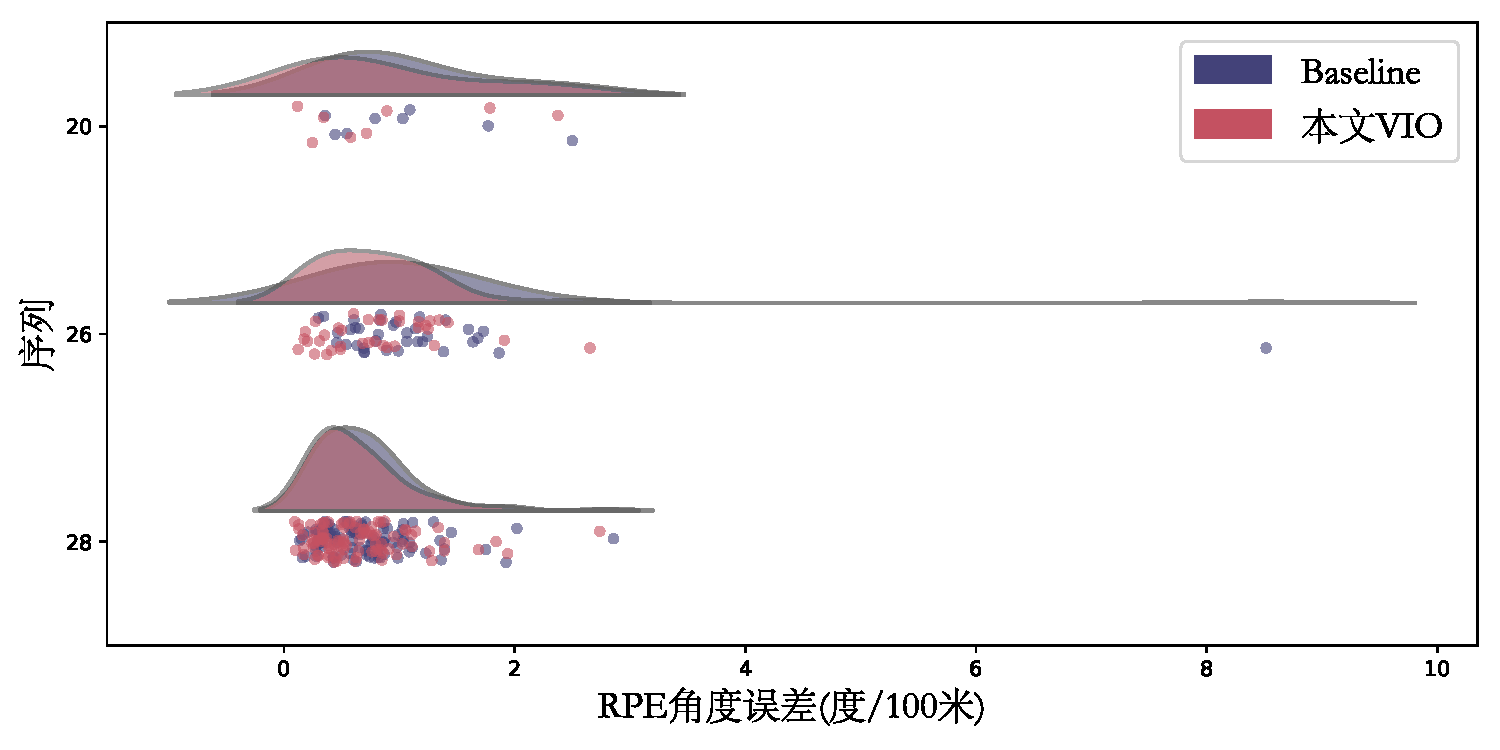
\includegraphics[width=1.0\linewidth]{kaist_cloud.pdf}
  \caption{KAIST数据集上$RPE_r$\textdownarrow{}分布示意图}
  \label{fig:vio_kaist}
\end{figure}

从表中可以看出,本文设计的PO-VIO在大部分序列上均取得了误差上的改进。对于20-Highway序列,经过改进后,绝对轨迹误差($ATE_t$)从27.55降至26.00,每公里降低约1.55;旋转误差($RPE_r$)也由1.17降低到0.69,减少了约0.48,但相对平移误差($RPE_t$)则略有增加,从19.50上升至20.16。对于26-Dongtan 序列,改进后的$ATE_t$由6.92降至6.46,$RPE_t$从8.91降低到6.54,$RPE_r$也由1.58降低到0.97,三项指标均有明显改善。28-Pangyo序列中,$ATE_t$由5.12降至4.59,$RPE_t$则显著从11.80下降到8.79,而$RPE_r$变化较小,从0.81略降至0.78。

总体来看,尽管20-Highway序列中$RPE_t$有所上升,但本文设计在大部分场景下均能有效降低绝对及相对误差,整体性能得到了提升。

为了展示本文设计的PO-VIO与基线的稳定性效果对比,本文在图~\ref{fig:vio_kaist} 中展示了KAIST数据集上$RPE_r$\textdownarrow{}的分布情况。从图中可以看出,本文的PO-VIO在KAIST数据集上的$RPE_r$\textdownarrow{}分布更加集中,且均值更低,相较于基线有着更好的效果。

\subsection{PO-VIO性能提升的来源分析}
针对PO-VIO性能提升的原因,本文猜测可能是因为本文所提出的伪观测约束项~\eqref{eq:imu_residual} 中仅存在有关旋转和速度的约束,并不直接对平移进行约束,所以在相对平移误差上表现较差,而在相对旋转误差上表现较好。

为了验证这一猜想,本文对车身坐标系的速度量进行分析。分析建立在OF2和OF3两条序列上,这两条序列有着比较突出的特点:OF2序列上本文PO-VIO的$RPE_t$和$RPE_r$均有所提升,但是整体幅度较小;OF3序列上本文PO-VIO的$RPE_t$有所下降,但是$RPE_r$有所提升,而且每100米的旋转误差减小了接近1$\degree$/100m。因此选择这两条序列进行分析,能够更好发现本文的速度伪观测约束在何种条件下会对里程计的效果产生积极影响。两条序列上的速度量在车身坐标系的变化如图~\ref{fig:VIO_velocity} 所示。

\begin{figure}
  \centering
  \subcaptionbox*{OF2序列}{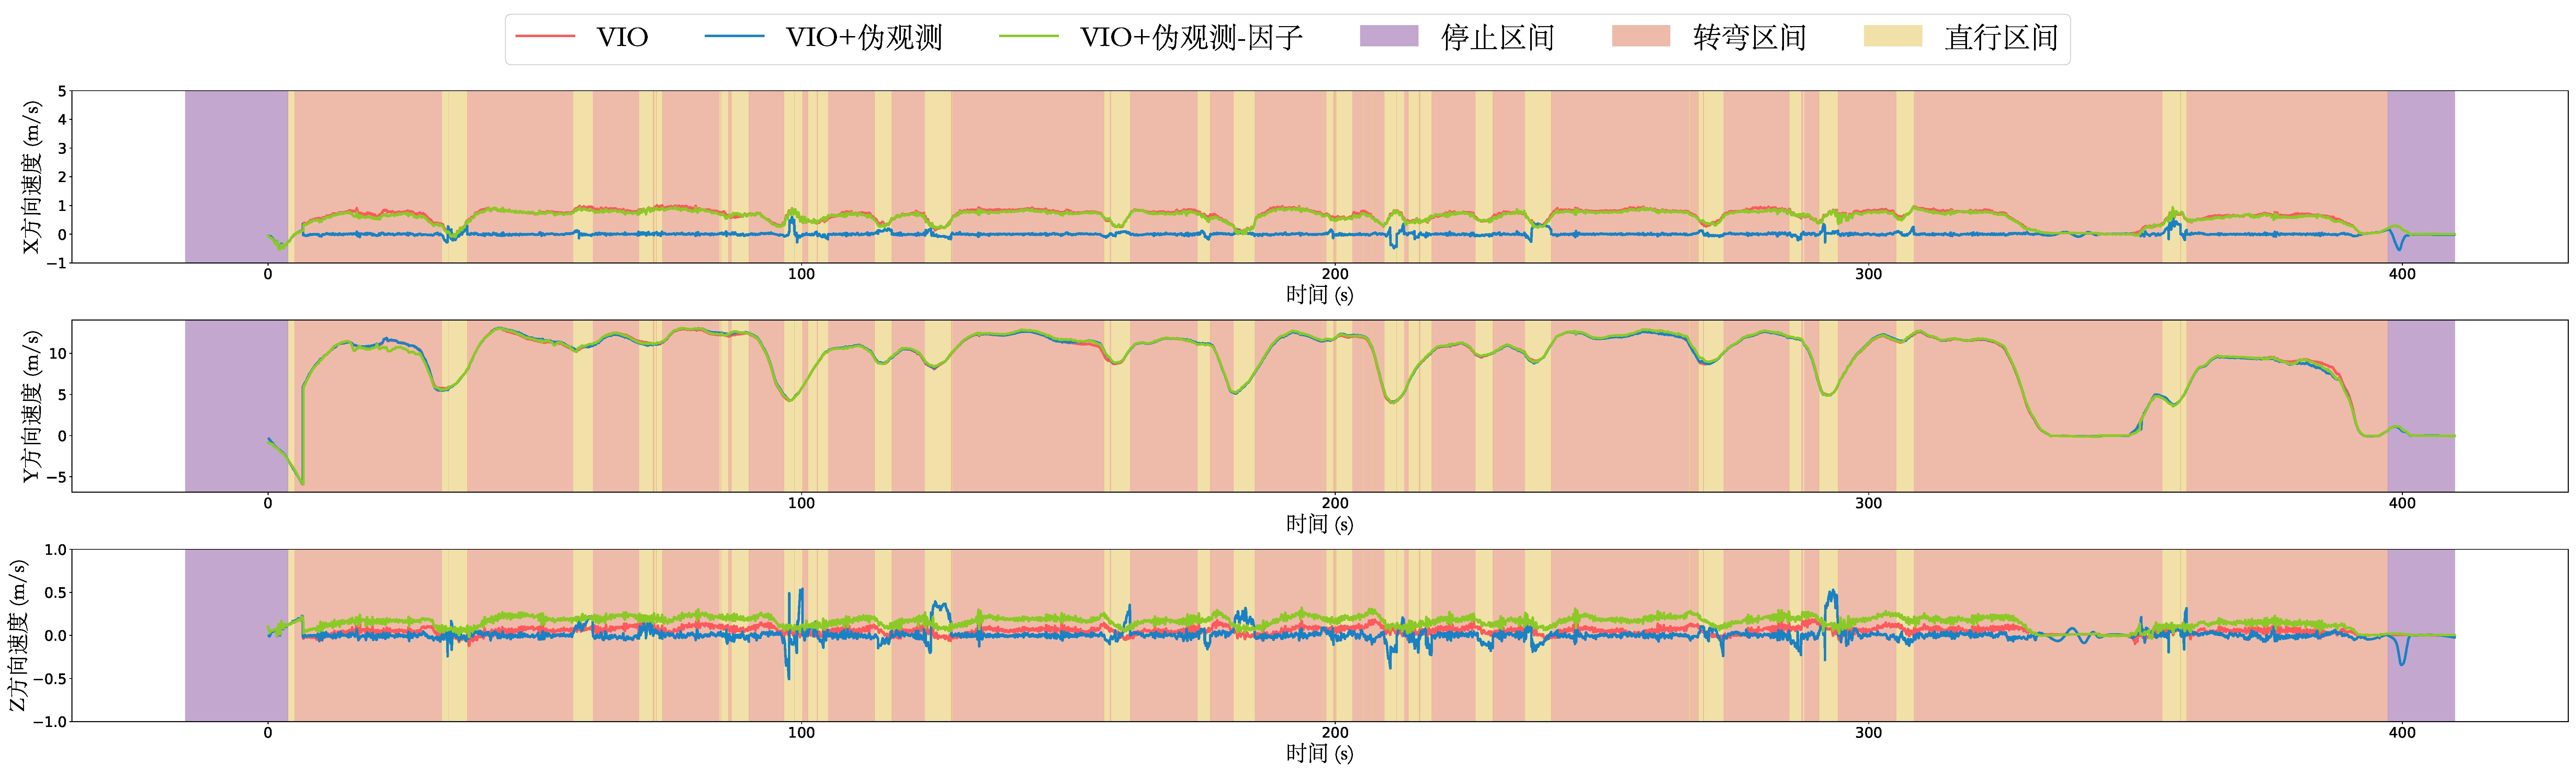
\includegraphics[width=1.0\linewidth]{VIO_velocity_OF2.pdf}}
  \subcaptionbox*{OF3序列}{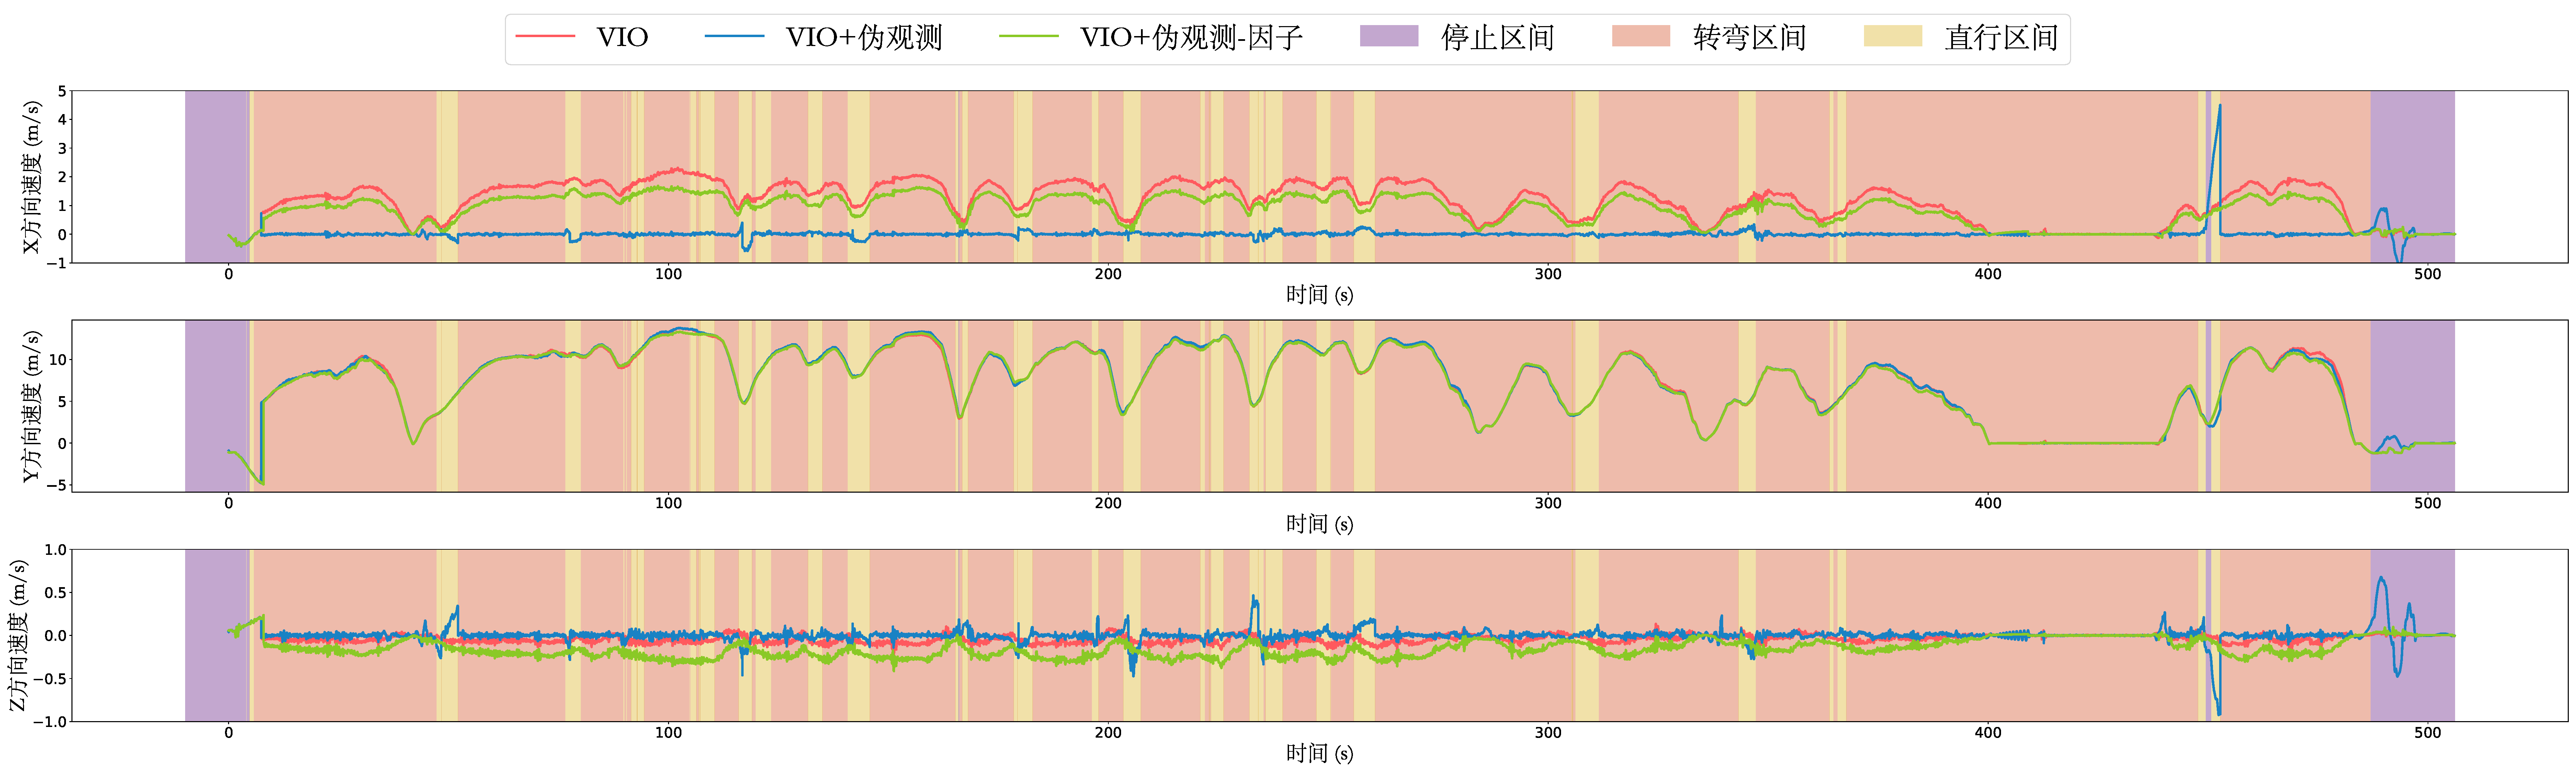
\includegraphics[width=1.0\linewidth]{VIO_velocity_OF3.pdf}}
  \caption{车身速度展示}
  \label{fig:VIO_velocity}
\end{figure}

在每个序列上分别展示了“VIO”、“VIO+伪观测”、“VIO+伪观测-因子”三种情况下的速度变化,其中“VIO”表示使用通用VIO方法获得的速度估计结果;“VIO+伪观测”表示在通用VIO中加入本文所提出的车身状态判断以及伪观测约束后的速度估计结果;“VIO+伪观测-因子”表示在VIO和伪观测约束的基础上,不使用惯性-车体因子进行后端优化。此外,为了将速度变化与车身状态区间直观展示,本文中还将对应车身停止、转弯和直行的区间标注在了速度图中。

从两个序列中的速度变化可以看到:相较于OF2序列,OF3序列的“VIO”在车身横向(X轴方向)和垂直(Z轴方向)速度上有着更大的取值,这说明在OF3序列上基础VIO的速度估计有更大的误差,而在该场景下,经过本文所提出的伪观测约束进行优化后,“VIO+伪观测”横向和垂直速度有了更合理的估计,从而使得OF3上的$RPE_r$有了明显的提升。相较而言,OF2序列上的速度变化较为平缓,所以在该场景下,伪观测约束的加入对于速度估计的影响较小,使得“VIO+伪观测”在OF2序列上的$RPE_r$仅有微弱提升。

此外,观察两个序列下的速度变化,可以发现在OF2上,“VIO+伪观测”的车身横向和垂直速度全过程都有较为平滑的估计结果,相比之下OF3序列上“VIO+伪观测”在最后阶段出现了较明显的起伏,因此其出现了OF3序列上本文方法的$RPE_t$有所下降的现象,而OF2序列上本文方法的$RPE_t$达到同类方法的最优。


\subsection{消融实验}
为了探究本文提出的VIO方法中各个模块的效果,本文进行了消融实验,消融实验在OF3序列上进行,选择控制的变量包括“VIO”、“惯性-车体因子”、“伪观测约束”、“车身状态判别”和“车身状态真值”,其中“VIO”是基础配置,其他变量的加入均是在VIO的基础上进行的;“惯性-车体因子”表示是否在后端窗口优化时将惯性-车体对齐参数作为优化变量;“伪观测约束”表示是否在后端窗口优化时加入含有伪观测约束的IMU残差;“车身状态判别”表示是否根据车身状态判别神经网络的结果而调整后端优化量;“车身状态真值”表示是否根据车身状态的真值而调整后端优化量,其可以看做是车身状态判别的上限。实验结果如表~\ref{tab:vio_ablation} 所示。表中展示了在不同消融实验下的$ATE_t$、$RPE_t$和$RPE_r$的结果,其中$\checkmark$表示使用了对应的模块。

\begin{table}
\centering
\caption{PO-VIO消融实验}
\begin{tabular}{cccccccc}
\toprule
VIO        & \begin{tabular}[c]{@{}c@{}}惯性-车体\\ 因子\end{tabular} & \begin{tabular}[c]{@{}c@{}}伪观测\\ 约束\end{tabular} & \begin{tabular}[c]{@{}c@{}}车身状态\\ 判别\end{tabular} & \begin{tabular}[c]{@{}c@{}}车身状态\\ 真值\end{tabular} & $ATE_t$\textdownarrow{}       & $RPE_t$\textdownarrow{}     & $RPE_r$\textdownarrow{}      \\ \midrule
$\checkmark$           &                          &                        &                         &                         & 20.552186            & 5.648737             & 3.411987             \\
$\checkmark$           & $\checkmark$               & $\checkmark$             &                         &                         & 23.269810            & 5.594315             & 2.588779             \\
$\checkmark$           & $\checkmark$               & $\checkmark$             & $\checkmark$              &                         & 17.193425            & 5.887755             & 2.543815             \\
$\checkmark$           & $\checkmark$               & $\checkmark$             &                         & $\checkmark$              & 14.685789            & 5.277349             & 2.522826             \\
$\checkmark$           &                          & $\checkmark$             &                         & $\checkmark$              & 17.361096            & 5.099256             & 2.577359             \\ \bottomrule
\end{tabular}
\label{tab:vio_ablation}
\end{table}

表中第二行的含义是不论车身处于何种状态,均使用直行时的车身速度假设,因此从前两行的对比中可以发现,当使用了惯性车体因子和伪观测约束后,$ATE_t$产生了明显的下降,但是$RPE_t$有了轻微的改善,$RPE_r$有了明显的改善。这说明了惯性车体因子和伪观测约束的加入对于车身旋转的估计有着重要的影响,但是这会对平移的估计产生一定负面影响。即说明如果全程使用直行时的车身速度假设,会对里程计的平移估计精度产生负面影响,但对旋转的估计精度有积极影响。

表中第三行在第二行的基础上加入了对车身状态的预测,虽然预测与真实情况可能存在偏差,但是可以从数据上得出:当加入了车身状态判别后,$ATE_t$产生明显的下降,$RPE_t$有所增加,$RPE_r$有轻微改善,这说明了车身状态判别对于绝对定位精度的提升有着重要的影响。虽然其本身存在的状态预测误差则会对相对位移的估计产生一定的负面影响,但是综合来看其对于绝对位置和旋转角度估计的精度提升可以使其忽略对相对位移估计产生的负面影响。

表中第四行在第三行的基础上将车身状态的预测值替换为真值,这一行为对$ATE_t$、$RPE_t$和$RPE_r$三个指标都产生了增益效果,这侧面证明了:当使用预测值时产生的相对位移估计精度损失是由于预测值的误差导致的,而当使用真值时,这一误差被消除,所以在$ATE_t$、$RPE_t$和$RPE_r$三个指标上都取得了较大的进步。

表中最后一行在第四行的基础上去掉了惯性车体因子,即在优化过程中不优化惯性-车体因子,而仅使用初始量。这一行相较于第四行的结果是:$ATE_t$和$RPE_r$产生了一定程度的损失,但是$RPE_t$却达到了最好效果。这一行的结果表明:惯性-车体因子的实时优化对于绝对位置精度和旋转估计有着重要的积极影响,但是对于相对平移估计则有着负面影响。但是综合来看,优化惯性-车体因子对于绝对位置和相对旋转的估计的提升明显,而对于相对位置估计精度的影响有限,因此有保留的必要。

\section{地图定位模块测试}
地图定位模块的测试在KITTI数据集和4Seasons数据集上进行,本节将分别对两个数据集上的测试结果进行展示。其中KITTI数据集上的测试使用模拟的多趟行驶数据,建图场景和测试场景的变化较小;而4Seasons数据集上的测试使用真实的多趟行驶数据,定位和建图的场景变化较大,具有较强的挑战性。

\subsection{精度测试}
\subsubsection{KITTI数据集测试}
在KITTI数据集上,本文的地图定位模块测试结果如图~\ref{fig:loc_kitti} 和表~\ref{tab:loc_kitti} 所示,在表~\ref{tab:loc_kitti} 中以加粗字体和红底标出最佳表现。

\begin{figure}
  \centering
  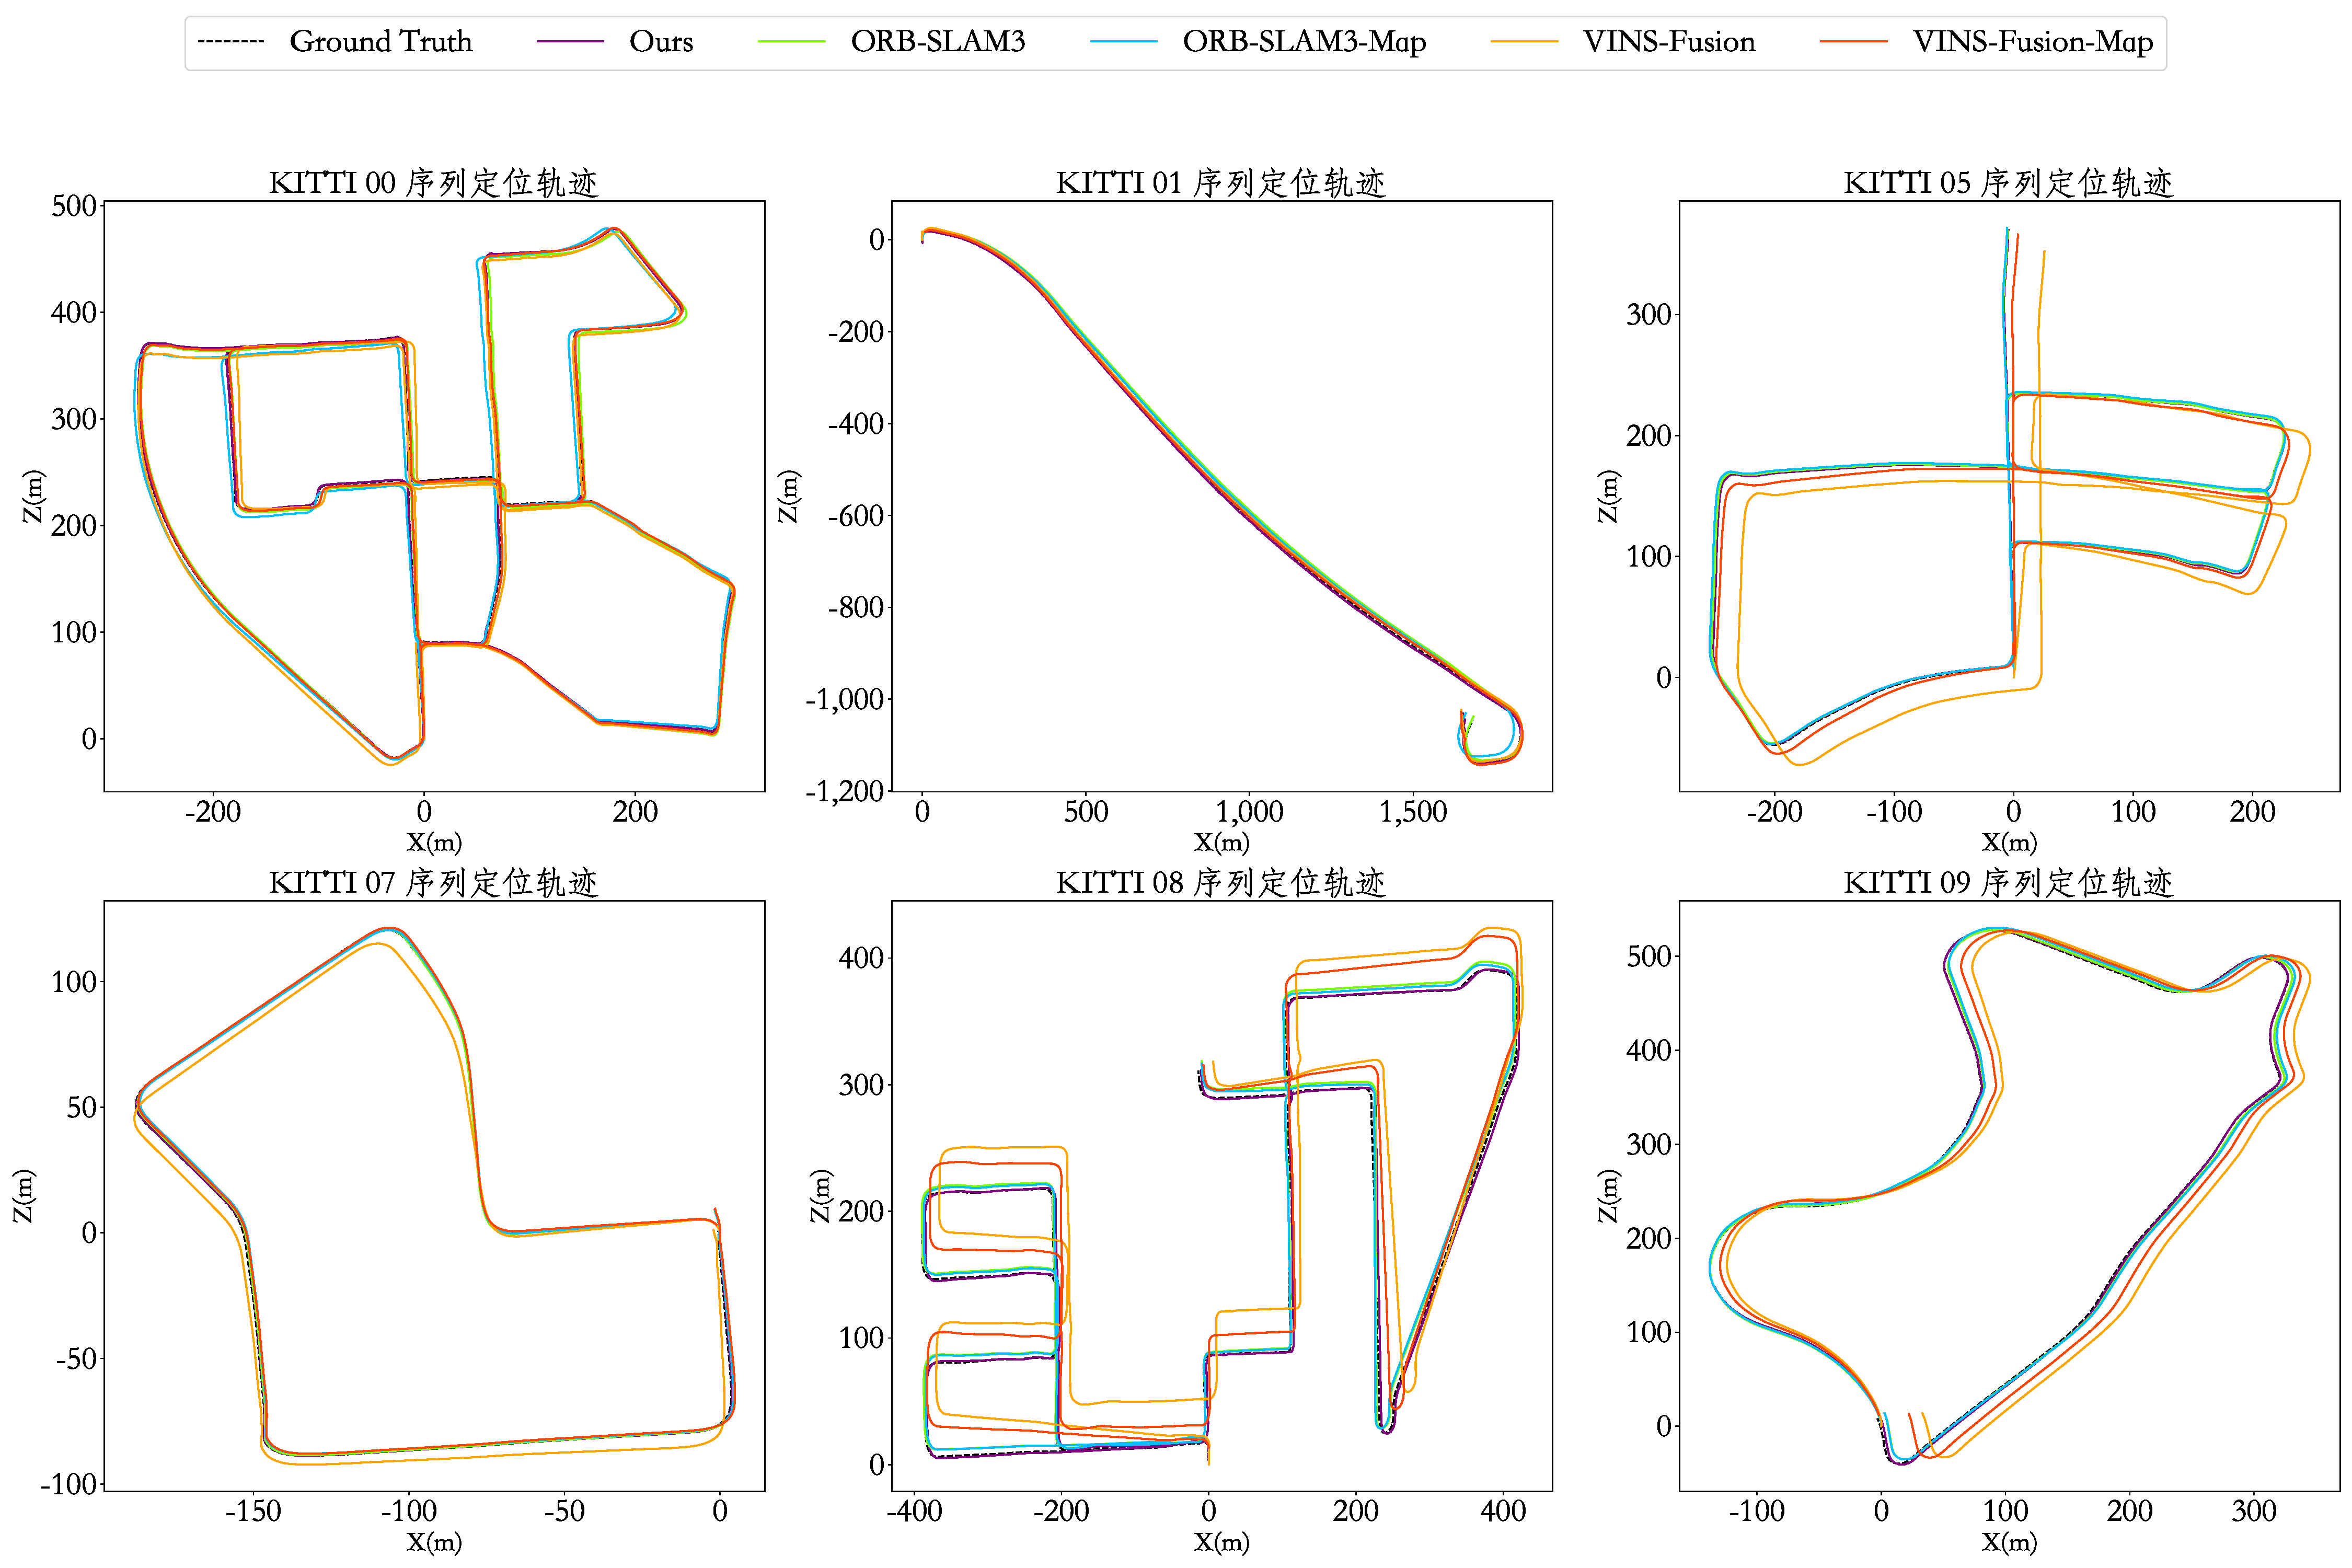
\includegraphics[width=1.0\linewidth]{loc_kitti.pdf}
  \caption{KITTI数据集测试轨迹示意图}
  \label{fig:loc_kitti}
\end{figure}

对比的方法包括VINS-Fusion(VINS)、VINS-Fusion-Map(VINSM)、ORB-SLAM3(ORB)和ORB-SLAM3-Map(ORBM)进行对比,其中VINS-Fusion-Map和ORB-SLAM3-Map是VINS-Fusion和ORB-SLAM3的地图版本。

\begin{table}
\centering
\begin{threeparttable}
\caption{KITTI数据集多指标对比}
\begin{tabular}{lccccccccccc}
\toprule
方法    & 指标                    & 00            & 01            & 02            & 04            & 05            & 06            & 07            & 08            & 09            & 10            \\ \midrule
ORB   & \multirow{5}{*}{$ATE_t$\textdownarrow{}}  & 3.51          & 4.92          & 5.70          & \cellcolor[HTML]{FFCCC9}\textbf{0.27} & 1.84          & 1.68          & 0.96          & 3.32          & 3.37          & 0.90          \\
ORBM  &                       & 7.19          & 10.11         & 10.32         & 0.98          & 1.54          & 2.35          & 1.67          & 5.36          & 7.61          & 0.95          \\
VINS  &                       & 5.95          & 6.49          & 5.99          & 1.08          & 5.98          & 3.48          & 2.41          & 3.85          & \cellcolor[HTML]{FFCCC9}\textbf{1.78}          & 3.78          \\
VINSM &                       & 3.92          & 8.01          & 13.08         & 1.23          & 3.88          & 1.79          & 0.65          & 9.89          & 6.17          & 3.63          \\
本文方法    &                       & \cellcolor[HTML]{FFCCC9}\textbf{0.97} & \cellcolor[HTML]{FFCCC9}\textbf{4.09} & \cellcolor[HTML]{FFCCC9}\textbf{0.70} & 0.53          & \cellcolor[HTML]{FFCCC9}\textbf{1.24} & \cellcolor[HTML]{FFCCC9}\textbf{1.56} & \cellcolor[HTML]{FFCCC9}\textbf{0.21} & \cellcolor[HTML]{FFCCC9}\textbf{1.68} & 1.87 & \cellcolor[HTML]{FFCCC9}\textbf{0.82} \\ \midrule
ORB   & \multirow{5}{*}{$RPE_t$\textdownarrow{}} & 0.88          & 1.44          & 0.77          & \cellcolor[HTML]{FFCCC9}\textbf{0.46} & 0.62          & 0.89          & 0.89          & 1.03          & \cellcolor[HTML]{FFCCC9}\textbf{0.86} & 0.62          \\
ORBM  &                       & 0.69          & 1.46          & 0.77          & 0.49          & \cellcolor[HTML]{FFCCC9}\textbf{0.40} & \cellcolor[HTML]{FFCCC9}\textbf{0.46} & 0.52          & 1.04          & 0.87          & \cellcolor[HTML]{FFCCC9}\textbf{0.61} \\
VINS  &                       & 3.45          & 12.18         & 2.65          & 2.71          & 1.41          & 1.33          & 1.17          & 3.46          & 4.45          & 2.38          \\
VINSM &                       & 1.23          & 2.44          & 1.49          & 1.37          & 1.46          & 0.88          & 0.71          & 1.66          & 1.97          & 2.45          \\
本文方法    &                       & \cellcolor[HTML]{FFCCC9}\textbf{0.74} & \cellcolor[HTML]{FFCCC9}\textbf{1.44} & \cellcolor[HTML]{FFCCC9}\textbf{0.68} & 1.87          & 0.75          & 0.84          & \cellcolor[HTML]{FFCCC9}\textbf{0.39} & \cellcolor[HTML]{FFCCC9}\textbf{0.96} & 1.03          & 0.82          \\ \midrule
ORB   & \multirow{5}{*}{$RPE_r$\textdownarrow{}} & 0.31          & \cellcolor[HTML]{FFCCC9}\textbf{0.19} & \cellcolor[HTML]{FFCCC9}\textbf{0.28} & 0.19          & 0.26          & 0.27          & 0.50          & 0.31          & 0.25          & 0.29          \\
ORBM  &                       & 0.26          & \cellcolor[HTML]{FFCCC9}\textbf{0.19} & \cellcolor[HTML]{FFCCC9}\textbf{0.28} & \cellcolor[HTML]{FFCCC9}\textbf{0.08} & \cellcolor[HTML]{FFCCC9}\textbf{0.16} & \cellcolor[HTML]{FFCCC9}\textbf{0.15} & 0.30          & 0.31          & 0.25          & \cellcolor[HTML]{FFCCC9}\textbf{0.28} \\
VINS  &                       & 1.45          & 3.54          & 1.26          & 0.62          & 0.69          & 0.72          & 0.87          & 1.77          & 1.87          & 0.94          \\
VINSM &                       & 0.73          & 0.48          & 0.56          & 0.69          & 0.67          & 0.58          & 0.57          & 0.65          & 0.59          & 0.99          \\
本文方法    &                       & \cellcolor[HTML]{FFCCC9}\textbf{0.27} & 0.34          & 0.30          & 0.30          & 0.19          & 0.17          & \cellcolor[HTML]{FFCCC9}\textbf{0.26} & \cellcolor[HTML]{FFCCC9}\textbf{0.29} & \cellcolor[HTML]{FFCCC9}\textbf{0.19} & 0.30          \\ \bottomrule
\end{tabular}
\label{tab:loc_kitti}
\begin{tablenotes}
  \item [a] ORB和ORBM分别表示ORB-SLAM3和ORB-SLAM3-Map
  \item [b] VINS和VINSM分别表示VINS-Fusion和VINS-Fusion-Map
\end{tablenotes}
\end{threeparttable}
\end{table}

从表中对KITTI数据集上多项指标的对比结果来看,不同方法在不同序列上表现存在较大差异。对于绝对轨迹误差$ATE_t$指标,本文方法在序列 00、01、02、05、06、07、08 和 10 上均取得了最低值,说明在绝对位姿精度上具有较明显的优势;仅在序列 04 上,ORB-SLAM3表现更优,而序列 09 的结果略有争议,尽管 VINS 在此处显示出稍低的误差,但总体来看,本文方法在大部分序列中均展现出更好的平稳性。

对于相对平移误差$RPE_t$而言,各方法的表现相对分散。本文方法在序列 01、02、07 和 08 上表现突出,但在其他序列中,ORB-SLAM3、ORB-SLAM3-Map或其他方法有时能获得更低的误差,表明在平移精度方面,各算法对场景和运动状态的敏感性不同。

而在相对旋转误差$RPE_r$方面,本文方法在部分序列,如 00、07、08、09,中取得了较低的值,体现出在角度估计上的一定优势,但在序列 01、02 和 04 上,ORB-SLAM3 或 ORB-SLAM3-Map 的表现更佳,说明在旋转精度上,算法之间仍存在细微差距。

综合来看,本文方法在大部分场景下均能保持较高的翻译精度,并在旋转估计上具有竞争力,这表明所提出的算法具有较好的鲁棒性和适应性。


\subsubsection{综合(Office Loop)场景测试}
4Seasons数据集实在同一条线路上多次采集获得的,采集的时间跨度从几十分钟到一年,所以其场景相对于KITTI数据集有更多的变化,包括季节、天气、晨昏等。本文首先在Office Loop的一般性场景下进行测试。一般性场景测时的建图序列为2020.03.24 17:36拍摄,而定位序列为2020.03.24 17:45拍摄,两个场景差异较小,因此可以同时比较多个方法的表现。

\begin{table}
\centering
\begin{threeparttable}[c]
\caption{4Seasons数据集Office Loop场景第2序列指标对比}
\begin{tabular}{lccccccc}
\toprule
方法                                     & 时间                                                                         & 季节                   & 天气                   & 晨昏                   & $ATE_t$\textdownarrow{}               & $RPE_t$\textdownarrow{}              & $RPE_r$\textdownarrow{}              \\ \midrule
离线建图                                   & \begin{tabular}[c]{@{}c@{}}03.24\\ 17:36 \\ (OF1)\end{tabular}                   & 春季                   & 晴朗                   & 下午                   & 0.814881          & 0.929358          & 1.014480          \\ \midrule
VINS-Mono                              & \multirow{10}{*}{\begin{tabular}[c]{@{}c@{}}03.24\\ 17:45 \\ (OF2)\end{tabular}} & \multirow{10}{*}{春季} & \multirow{10}{*}{晴朗} & \multirow{10}{*}{下午} & 7.878626          & 2.330876          & 0.783557          \\
VINS-Mono w/ Map1                      &                                                                            &                      &                      &                      & 3.092430          & N/A               & N/A               \\
VINS-Monow/ Map2                       &                                                                            &                      &                      &                      & 2.440850          & N/A               & N/A               \\
ORB-SLAM3                              &                                                                            &                      &                      &                      & 15.621815         & 3.222846          & 0.890233          \\
ORB-SLAM3 w/ Map3                      &                                                                            &                      &                      &                      & 19.249121         & N/A               & N/A               \\
VINS-Fusion w/  RTK &                                                                            &                      &                      &                      & 1.801669          & 1.500405          & 1.085638          \\
VLS                                    &                                                                            &                      &                      &                      & 1.715343          & 1.630718          & \cellcolor[HTML]{FFCCC9}\textbf{0.668220} \\
GPLD                                   &                                                                            &                      &                      &                      & 8.720000          & N/A               & N/A               \\
MVIL                                   &                                                                            &                      &                      &                      & 6.450000          & N/A               & N/A               \\
本文方法                                   &                                                                            &                      &                      &                      & \cellcolor[HTML]{FFCCC9}\textbf{0.777091} & \cellcolor[HTML]{FFCCC9}\textbf{1.124076} & 0.759267          \\ \bottomrule
\end{tabular}
\label{tab:loc_4seasons_of2}
\begin{tablenotes}
  \item [a] Map1表示使用VINS-Mono建图结果
  \item [b] Map2表示使用本文离线建图结果
  \item [c] Map3表示使用ORB-SLAM3建图结果
  \item [d] RTK表示使用了RTK-GPS数据,其定位精度达到厘米级
\end{tablenotes}
\end{threeparttable}
\end{table}

测试结果如表~\ref{tab:loc_4seasons_of2} 所示,其中包括了VINS-Mono、VINS-Fusion w/ RTK、ORB-SLAM3、VLS\cite{yang2022real}(2022)、GPLD\cite{hao2023global}(2023)、MVIL\cite{zhang2023map}(2023)等方法与本文方法的对比,其中VINS-Fusion w/ RTK使用了高精度(厘米级)GNSS信号,而VLS、GPLD、MVIL则是近期涌现的三种基于地图的定位方法。

首先在OF1和OF2两个序列上进行实验,这两个序列由于拍摄时间接近,所以场景变化不大,因此在其中进行的实验还包括了VINS-Mono w/ Map1、VINS-Mono w/ Map2、ORB-SLAM3 w/ Map3等方法的对比。从表~\ref{tab:loc_4seasons_of2} 中可以看出,本文方法在$ATE_t$和$RPE_t$上均取得了最佳表现,而在$RPE_r$上略逊于VLS方法,此外本文方法是第一个将定位精度提升到1米以内的方法,本文将其在卫星图上的定位结果展示如图~\ref{fig:loc_4seasons_of2} 所示。

\begin{figure}
  \centering
  \subcaptionbox{OF1序列建图轨迹\label{fig:loc_4seasons_of1}}{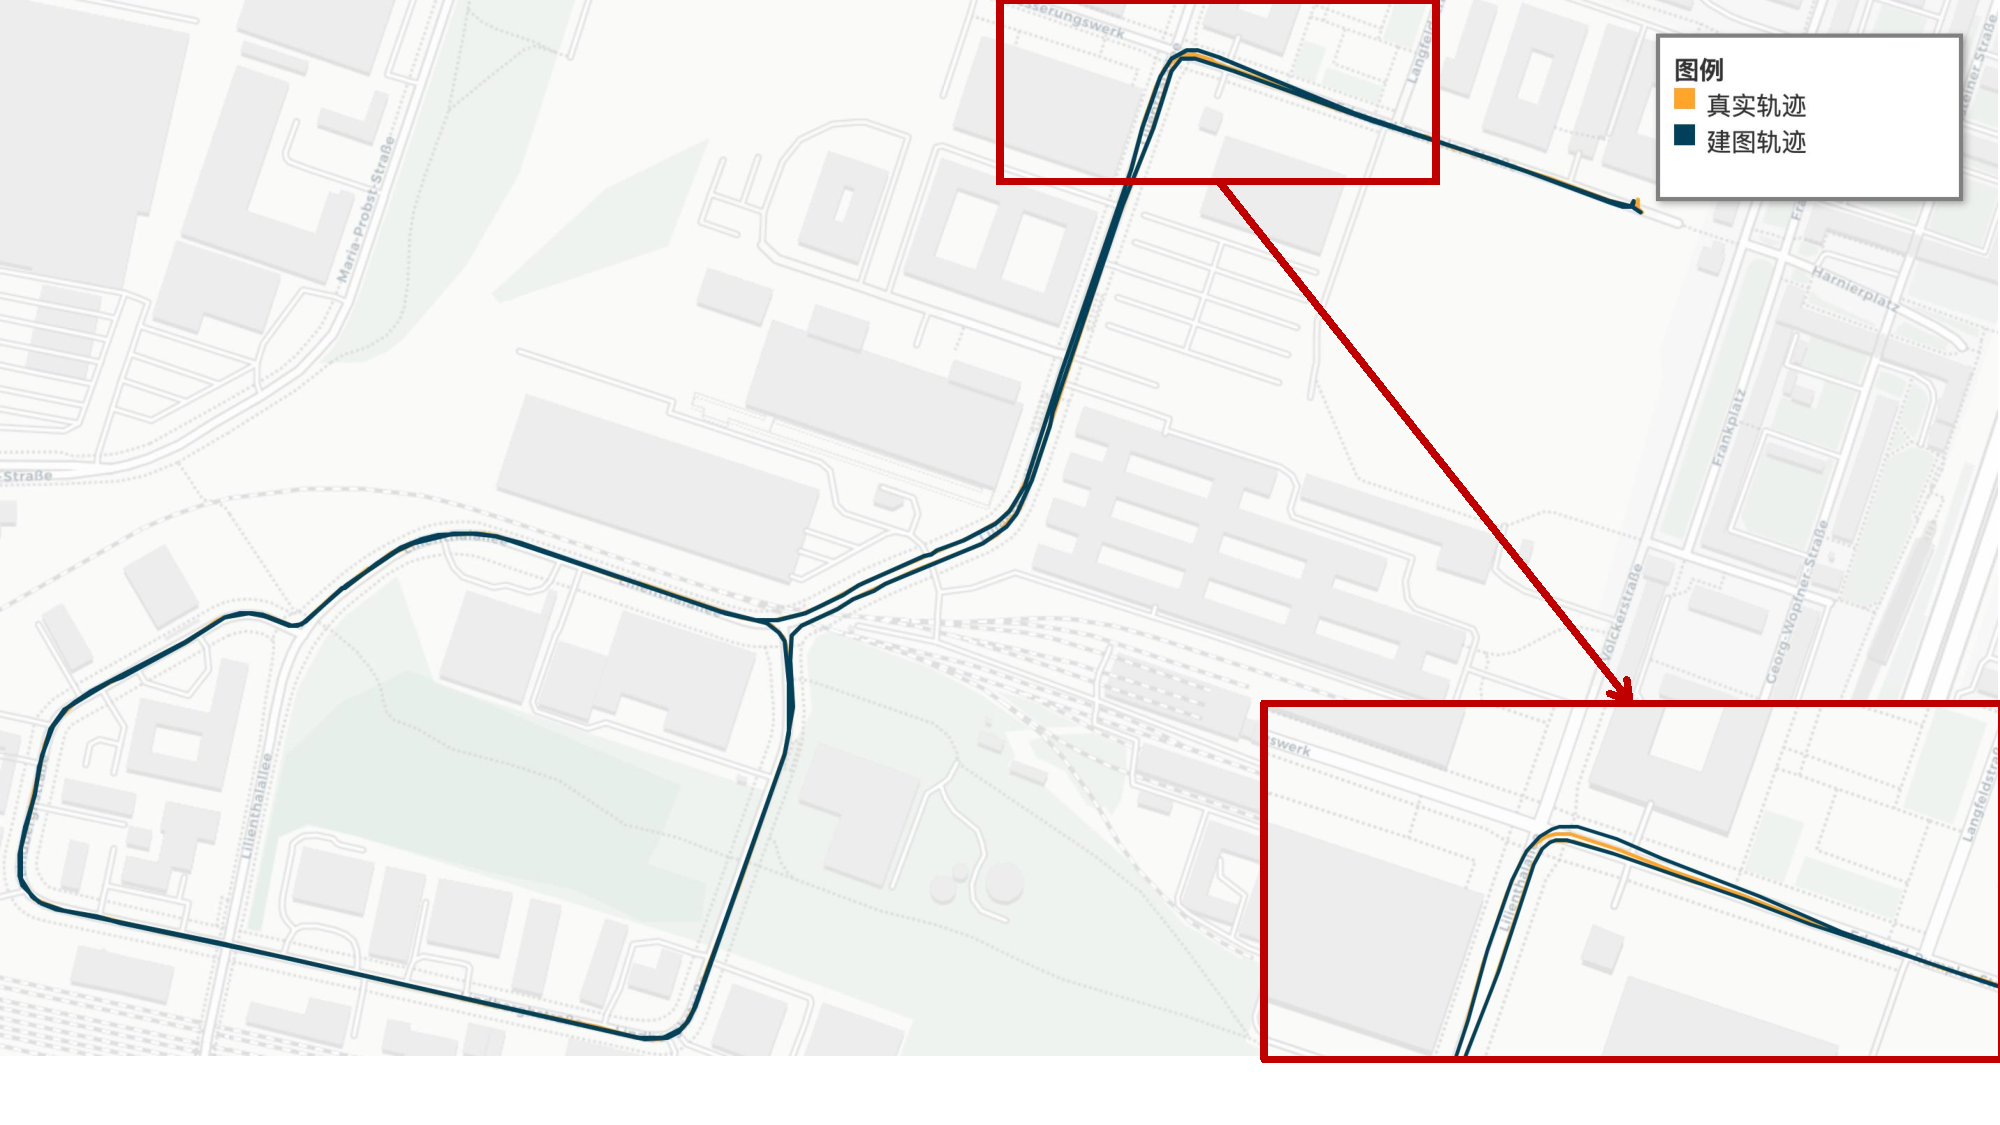
\includegraphics[width=0.47\linewidth]{OF1_zoomin.pdf}}
  \subcaptionbox{OF2序列定位轨迹\label{fig:loc_4seasons_of2}}{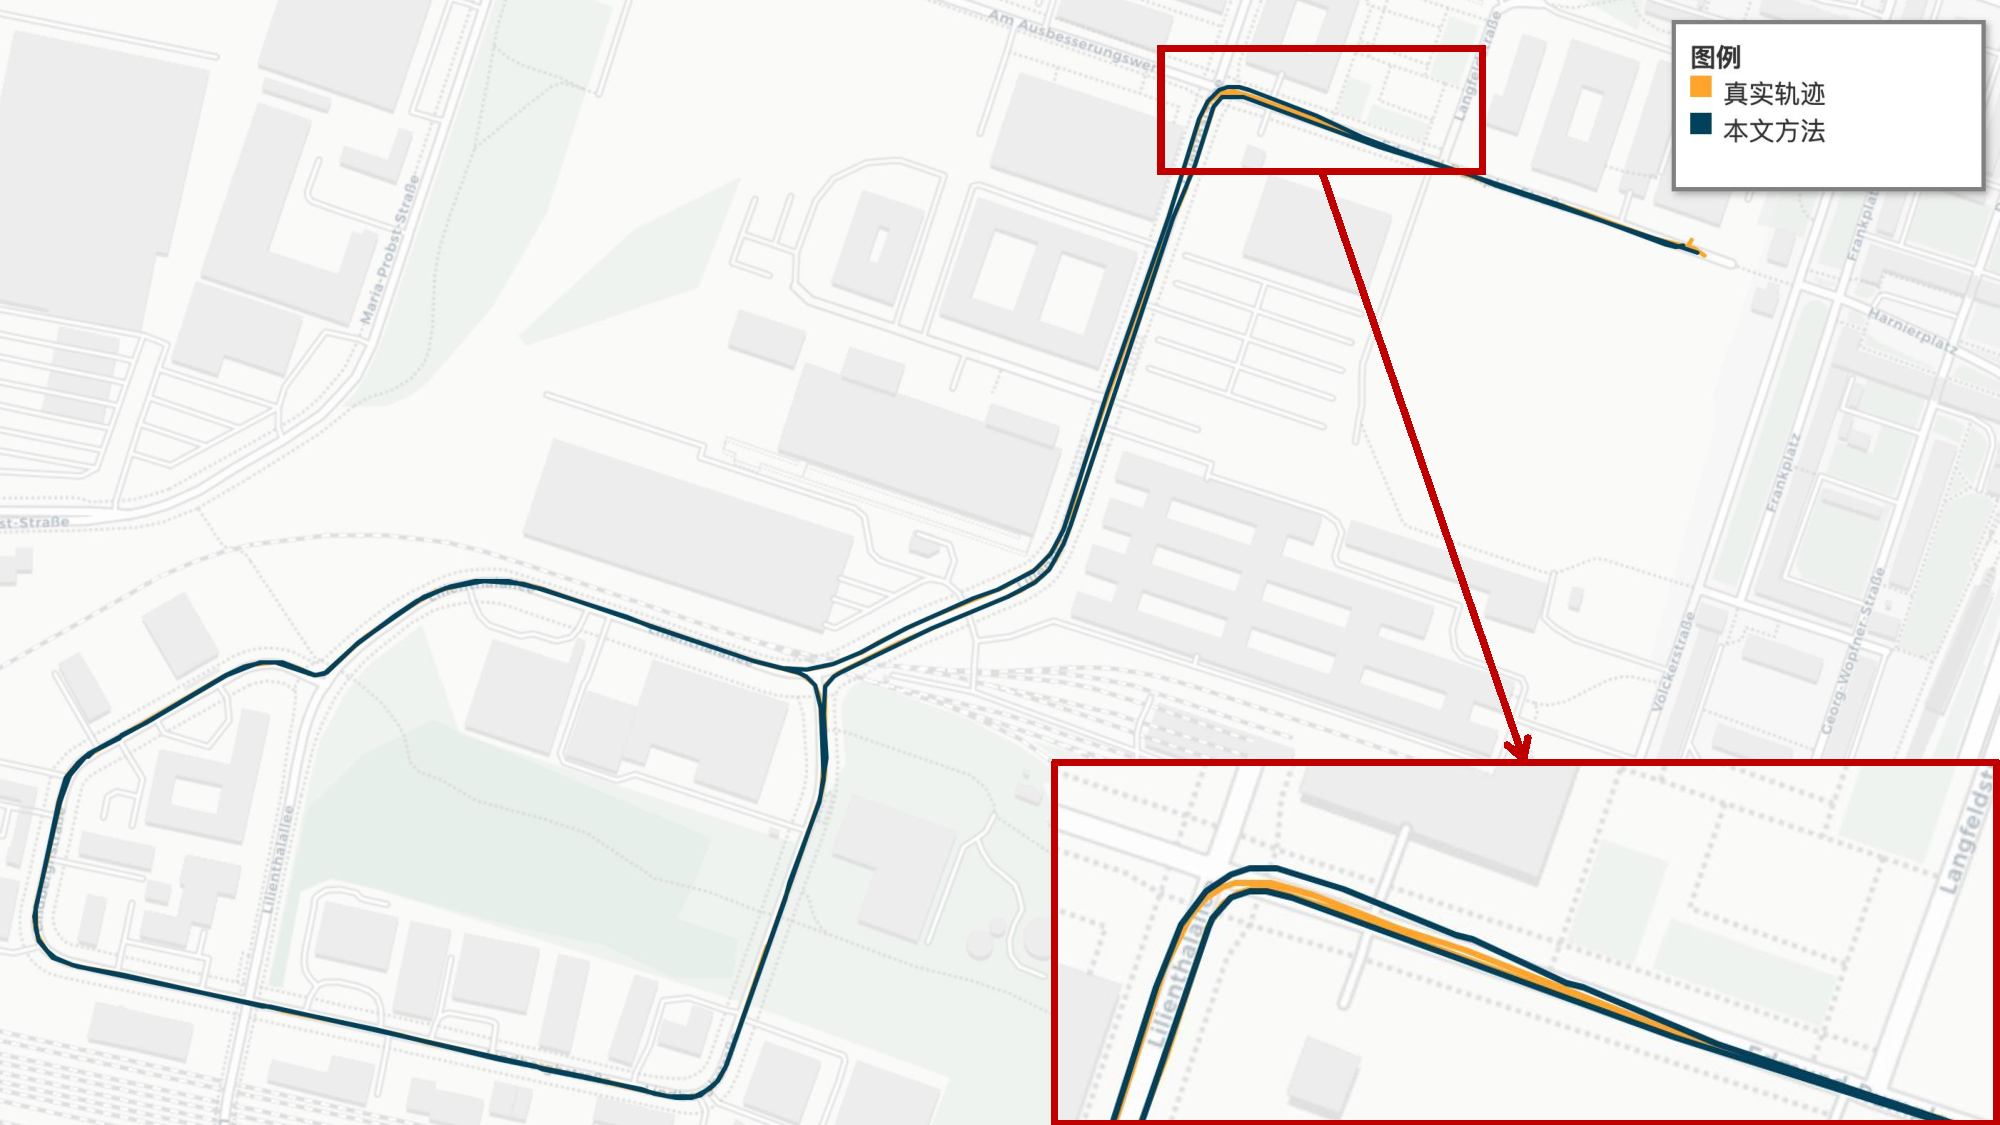
\includegraphics[width=0.45\linewidth]{OF2_zoomin.pdf}}
  \caption{4Seasons数据集定位结果及误差分析}
  \label{fig:loc_gnssmap}
\end{figure}

在图~\ref{fig:loc_4seasons_of2} 中可以看到在放大区域有着明显的定位误差,但这并非由于定位方法引入,而是由建图误差引入:如图~\ref{fig:loc_4seasons_of1} 所示,可以看到在定位误差较大的区域,建图时本身就存在明显的偏差,这导致了定位过程中引入了这一误差。因此,本文的定位方法在4Seasons数据集上的表现是受到了建图质量的影响,但是相较于其他方法,本文的定位方法在相同的建图条件下取得了更好的定位精度。

\begin{figure}
  \centering
  
\includegraphics[width=0.1\linewidth]{white.png}
  \subcaptionbox{OF1序列建图场景\label{fig:scene_of1}}{
    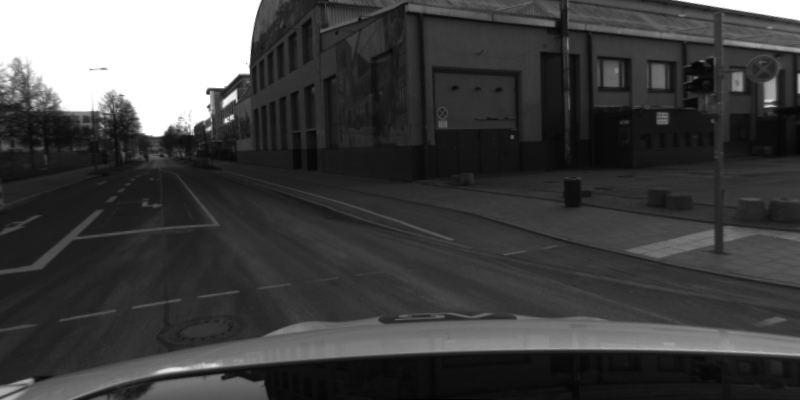
\includegraphics[width=0.32\linewidth]{OfficeLoop.png}
    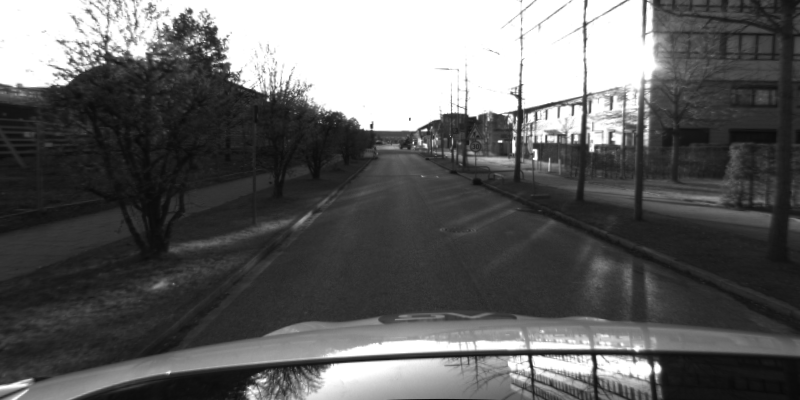
\includegraphics[width=0.32\linewidth]{OfficeLoop1_tree.png}}
  % 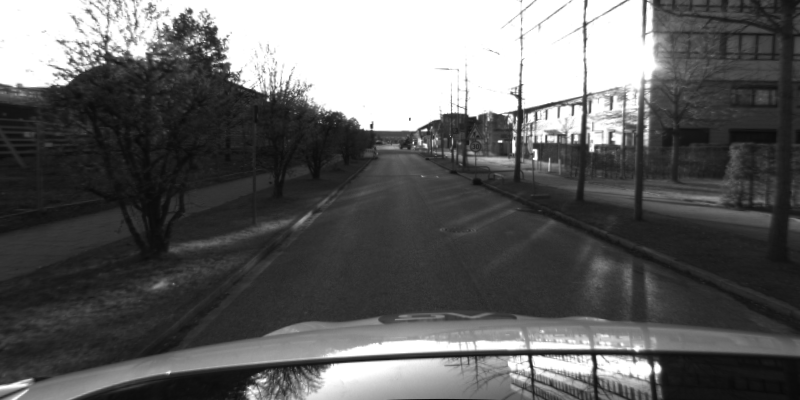
\includegraphics[width=0.32\linewidth]{OfficeLoop1_tree.png}
  
\includegraphics[width=0.1\linewidth]{white.png}
  \subcaptionbox{OF3序列清晨场景\label{fig:scene_of3}}{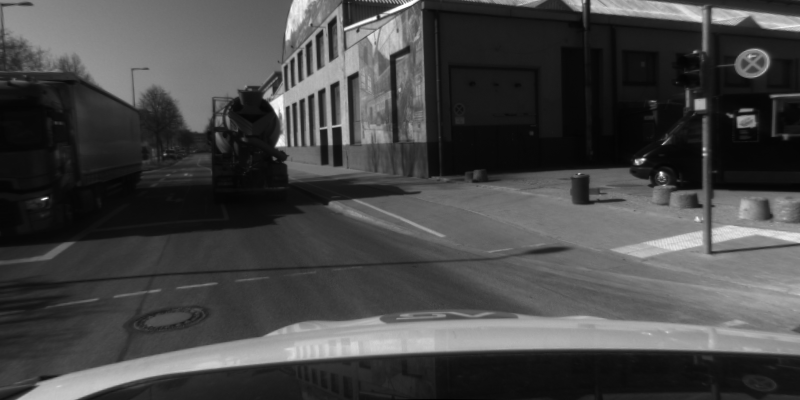
\includegraphics[width=0.32\linewidth]{OfficeLoop3.png}}
  \subcaptionbox{OF4序列夏季场景\label{fig:scene_of4}}{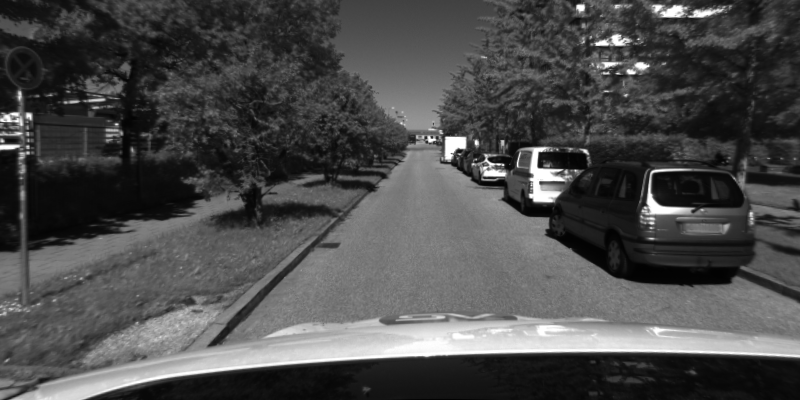
\includegraphics[width=0.32\linewidth]{OfficeLoop4.png}}
  \subcaptionbox{OF5序列冬季场景\label{fig:scene_of5}}{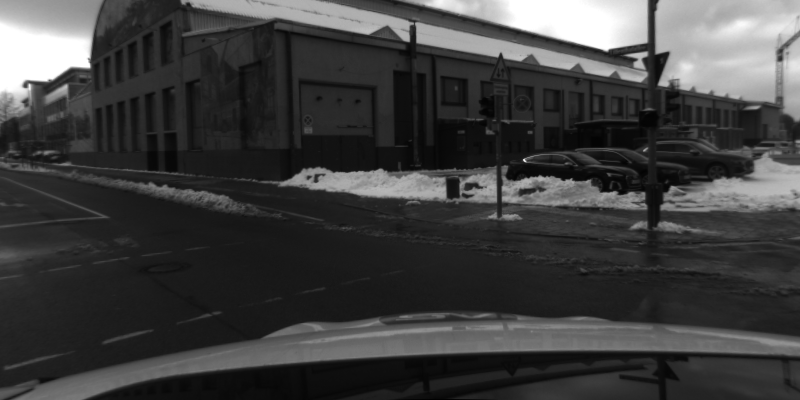
\includegraphics[width=0.32\linewidth]{OfficeLoop5.png}}
  \caption{4Seasons数据集OF3-5场景差异展示}
  \label{fig:scene_of}
\end{figure}

在Office Loop的环境下还有更多的具有挑战性的序列,本文在这些序列上也进行了测试。这些序列包括了OF3、OF4和OF5,具体的场景变化如图~\ref{fig:scene_of} 所示,这些序列的场景相较于OF2,有了晨昏~\ref{fig:scene_of3},季节~\ref{fig:scene_of4}和~\ref{fig:scene_of5},天气~\ref{fig:scene_of5} 的变化。定位的结果如表~\ref{tab:loc_4seasons_of345} 所示,需要说明的是,由于从OF3开始场景出现了较大的变化,因此一些使用传统方法的地图定位方法无法再依靠地图信息运行,因此此处仅汇报了可以运行的方法。

\begin{table}
\centering
\caption{4Seasons数据集Office Loop场景部分序列指标对比}
\begin{tabular}{lccccccc}
\toprule
方法                 & 时间                                                                             & 季节                  & 天气                  & 晨昏                  & $ATE_t$               & $RPE_t$              & $RPE_r$              \\ \midrule
离线建图               & \begin{tabular}[c]{@{}c@{}}03.24\\ 17:36\\ (OF1)\end{tabular}                  & 春季                  & 晴朗                  & 下午                  & 0.814881          & 0.929358          & 1.014480          \\ \midrule
VINS-Mono          & \multirow{5}{*}{\begin{tabular}[c]{@{}c@{}}04.07\\ 10:20\\ (OF3)\end{tabular}} & \multirow{5}{*}{春季} & \multirow{5}{*}{晴朗} & \multirow{5}{*}{清晨} & 10.664015         & 5.305404          & 5.305404          \\
ORB-SLAM3          &                                                                                &                     &                     &                     & 6.288431          & 5.000592          & 5.000592          \\
VINS-Fusion w/ RTK &                                                                                &                     &                     &                     & 2.000104          & 3.678773          & 3.678773          \\
VLS                &                                                                                &                     &                     &                     & 2.913034          & 3.978592          & 3.519618 \\
本文方法               &                                                                                &                     &                     &                     & \cellcolor[HTML]{FFCCC9}\textbf{0.938238} & \cellcolor[HTML]{FFCCC9}\textbf{2.947031} & \cellcolor[HTML]{FFCCC9}\textbf{2.529328} \\ \midrule
VINS-Mono          & \multirow{5}{*}{\begin{tabular}[c]{@{}c@{}}06.12\\ 10:10\\ (OF4)\end{tabular}} & \multirow{5}{*}{夏季} & \multirow{5}{*}{晴朗} & \multirow{5}{*}{清晨} & 7.661955          & 3.447067          & 1.747575          \\
ORB-SLAM3          &                                                                                &                     &                     &                     & 5.073350          & 3.207118          & 1.760357          \\
VINS-Fusion w/ RTK &                                                                                &                     &                     &                     & 1.809687          & 2.158715          & 1.577418          \\
VLS                &                                                                                &                     &                     &                     & 4.515426          & 8.142403          & 2.389229          \\
本文方法               &                                                                                &                     &                     &                     & \cellcolor[HTML]{FFCCC9}\textbf{0.792201} & \cellcolor[HTML]{FFCCC9}\textbf{1.402346} & \cellcolor[HTML]{FFCCC9}\textbf{1.047381} \\ \midrule
VINS-Mono          & \multirow{5}{*}{\begin{tabular}[c]{@{}c@{}}01.07\\ 12:04\\ (OF5)\end{tabular}} & \multirow{5}{*}{冬季} & \multirow{5}{*}{降雪} & \multirow{5}{*}{下午} & 8.083566          & 2.598062          & \cellcolor[HTML]{FFCCC9}\textbf{0.990526} \\
ORB-SLAM3          &                                                                                &                     &                     &                     & 5.520636          & 1.878826          & 1.000615          \\
VINS-Fusion w/ RTK &                                                                                &                     &                     &                     & 2.448607          & 1.333865          & 0.934714          \\
VLS                &                                                                                &                     &                     &                     & 1.862401          & 1.835533          & 0.999361          \\
本文方法               &                                                                                &                     &                     &                     & \cellcolor[HTML]{FFCCC9}\textbf{0.767040} & \cellcolor[HTML]{FFCCC9}\textbf{1.251208} & 0.999785          \\ \bottomrule
\end{tabular}
\label{tab:loc_4seasons_of345}
\end{table}

具体分析此场景下的不同序列可以看出,OF3和OF1两个序列的分别是在下午和清晨拍摄,所以图片中的光照强度首先就有一定的不同,此外图~\ref{fig:scene_of1} 和图~\ref{fig:scene_of3}中道路的车况也有一定区别,在图~\ref{fig:scene_of3} 中出现了建图过程未出现的车辆,为定位的细粒度特征匹配增加了较大困难。OF4和OF1两个序列存在季节的变化,从图~\ref{fig:scene_of1} 和图~\ref{fig:scene_of4} 中可以看到,OF4中的场景中出现了更繁茂的植被,甚至遮盖了部分建筑物,这对于细粒度特征匹配和定位都带来了一定的困难。OF5和OF1两个序列存在天气的变化,从图~\ref{fig:scene_of1} 和图~\ref{fig:scene_of5} 中可以看到,OF5中的场景中出现了降雪,改变了整个场景的整体感知条件,这对于定位的粗粒度和细粒度匹配都带来的挑战。

从表中信息可以看出:本文方法在所有序列的$ATE_t$和$RPE_t$指标上均取得了明显的优势,是所有方法中唯一误差稳定在1米以内的方法;在OF5上的$RPE_r$指标上略逊于VLS方法,但是差距极小。

在表~\ref{tab:loc_4seasons_of2} 和表~\ref{tab:loc_4seasons_of345} 中还可以发现本文方法在地图本身具有误差的情况下,定位结果却出现了部分超越地图精度的情况。这一现象结合后文的消融实验可以看到本文将地图建模为概率地图的做法具有一定作用:在地图中引入了不确定性后,紧耦合优化可以更好地利用地图信息,从而提升定位精度。


\subsubsection{低结构化(Neighborhood)场景测试}


Neighborhood场景中有更多的植被,接近于农村环境,因此在这个场景下的测试能表现出本文方法在较低纹理环境下的表现。在此场景下又增加了几种Office Loop场景中没有出现的条件,例如降雨天气(NH3)和傍晚环境(NH7)。测试结果如表~\ref{tab:loc_4seasons_nh23} 和表~\ref{tab:loc_4seasons_nh47}所示。

\begin{table}
\centering
\caption{4Seasons数据集Neighborhood场景第2与第3序列指标对比}
\begin{tabular}{lccccccc}
\toprule
方法                 & 时间                                                                             & 季节                  & 天气                  & 晨昏                  & $ATE_t$\textdownarrow{}               & $RPE_t$\textdownarrow{}              & $RPE_r$\textdownarrow{}              \\ \midrule
离线建图               & \begin{tabular}[c]{@{}c@{}}03.26\\ 13:32\\ (NH1)\end{tabular}                  & 春季                  & 多云                  & 下午                  & 0.133943          & 0.400299          & 0.451671          \\ \midrule
ORB-SLAM3          & \multirow{4}{*}{\begin{tabular}[c]{@{}c@{}}10.07\\ 14:47\\ (NH2)\end{tabular}} & \multirow{4}{*}{秋季} & \multirow{4}{*}{多云} & \multirow{4}{*}{下午} & 3.896760          & 1.177058          & \cellcolor[HTML]{FFCCC9}\textbf{0.957432} \\
VINS-Fusion w/ RTK &                                                                                &                     &                     &                     & 0.584860          & 2.081065          & 1.764747          \\
VLS                &                                                                                &                     &                     &                     & 0.385877          & \cellcolor[HTML]{FFCCC9}\textbf{1.015101}          & 1.005846 \\
本文方法               &                                                                                &                     &                     &                     & \cellcolor[HTML]{FFCCC9}\textbf{0.325610} & 1.079635 & 1.022361          \\ \midrule
ORB-SLAM3          & \multirow{4}{*}{\begin{tabular}[c]{@{}c@{}}10.07\\ 14:53\\ (NH3)\end{tabular}} & \multirow{4}{*}{秋季} & \multirow{4}{*}{降雨} & \multirow{4}{*}{下午} & 1.074461          & 1.193234          & \cellcolor[HTML]{FFCCC9}\textbf{0.980104} \\
VINS-Fusion w/ RTK &                                                                                &                     &                     &                     & 0.557219          & 1.922972          & 1.199615          \\
VLS                &                                                                                &                     &                     &                     & 0.338285          & 1.033000          & 1.002556          \\
本文方法               &                                                                                &                     &                     &                     & \cellcolor[HTML]{FFCCC9}\textbf{0.323113} & \cellcolor[HTML]{FFCCC9}\textbf{1.006227} & 1.006227          \\ \bottomrule
\end{tabular}
\label{tab:loc_4seasons_nh23}
\end{table}

降雨条件和傍晚条件的感知条件如图~\ref{fig:scene_nh} 所示,左图的降雨条件可以看到明显的水雾出现在图像上,而右图的傍晚环境,可以看到明显的亮度降低。在这种条件下本文方法依旧在所有序列的$ATE_t$和$RPE_t$指标上取得了最好的效果;虽然在$RPE_r$依旧没有比其他方法有明显优势,但是所有方法在该指标上的差距都非常小,更进一步展示了本文方法对环境的适应性。

\begin{figure}
  \centering
  \subcaptionbox*{NH3序列降雨场景\label{fig:scene_nh3}}{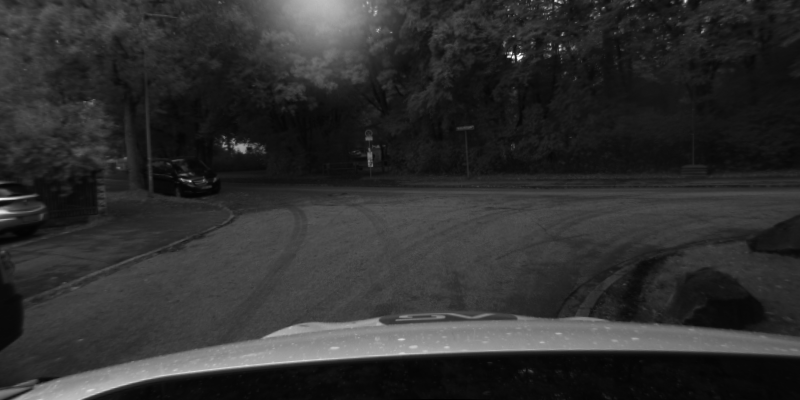
\includegraphics[width=0.32\linewidth]{Neighborhood3.png}}
  \subcaptionbox*{NH7序列傍晚场景\label{fig:scene_nh7}}{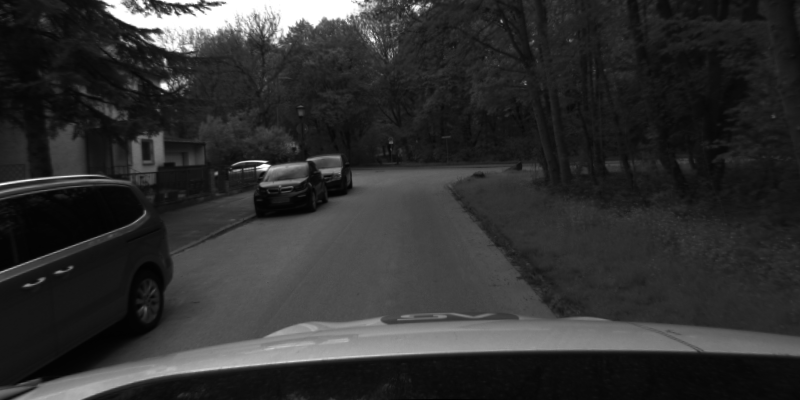
\includegraphics[width=0.32\linewidth]{Neighborhood7.png}}
  \caption{4Seasons数据集NH3与NH7场景差异展示}
  \label{fig:scene_nh}
\end{figure}

在此场景下由于离线建图的精度较高,因此本文方法在定位过程中能够更好地利用地图信息,从而提升定位精度,$ATE_t$指标下都获得了30厘米左右的误差,已经达到了厘米级的定位精度。但是此场景下,本文定位方法并没有出现超越地图精度的情况,这主要是受限于本文定位方法的精度上限,这一上限也将在后文的消融实验中进行验证。

\begin{table}
\centering
\caption{4Seasons数据集Neighborhood场景第4与第7序列指标对比}
\begin{tabular}{lccccccc}
\toprule
方法                 & 时间                                                                             & 季节                  & 天气                  & 晨昏                  & $ATE_t$\textdownarrow{}               & $RPE_t$\textdownarrow{}              & $RPE_r$\textdownarrow{}              \\ \midrule
离线建图               & \begin{tabular}[c]{@{}c@{}}03.26\\ 13:32\\ (NH1)\end{tabular}                  & 春季                  & 多云                  & 下午                  & 0.133943          & 0.400299          & 0.451671          \\ \midrule
ORB-SLAM3          & \multirow{4}{*}{\begin{tabular}[c]{@{}c@{}}12.22\\ 11:54\\ (NH4)\end{tabular}} & \multirow{4}{*}{冬季} & \multirow{4}{*}{多云} & \multirow{4}{*}{清晨} & 3.326053          & 1.721227          & 1.014069          \\
VINS-Fusion w/ RTK &                                                                                &                     &                     &                     & 0.584881          & 1.273095          & 1.337608          \\
VLS                &                                                                                &                     &                     &                     & 0.336795          & 0.828517          & \cellcolor[HTML]{FFCCC9}\textbf{0.722960} \\
本文方法               &                                                                                &                     &                     &                     & \cellcolor[HTML]{FFCCC9}\textbf{0.303237} & \cellcolor[HTML]{FFCCC9}\textbf{0.787774} & 0.793884          \\ \midrule
ORB-SLAM3          & \multirow{4}{*}{\begin{tabular}[c]{@{}c@{}}05.10\\ 18:32\\ (NH7)\end{tabular}} & \multirow{4}{*}{春季} & \multirow{4}{*}{多云} & \multirow{4}{*}{傍晚} & 1.770878          & 1.461675          & 1.239126          \\
VINS-Fusion w/ RTK &                                                                                &                     &                     &                     & 1.098182          & 3.455674          & 2.230523          \\
VLS                &                                                                                &                     &                     &                     & 0.304587          & 1.125579          & 1.007488          \\
本文方法               &                                                                                &                     &                     &                     & \cellcolor[HTML]{FFCCC9}\textbf{0.291957} & \cellcolor[HTML]{FFCCC9}\textbf{1.033805} & \cellcolor[HTML]{FFCCC9}\textbf{1.007318} \\ \bottomrule
\end{tabular}
\label{tab:loc_4seasons_nh47}
\end{table}

由于NH5和NH6所代表的场景已经出现在了表~\ref{tab:loc_4seasons_nh23} 和表~\ref{tab:loc_4seasons_nh47} 中,因此不再重复描述其具体数值,而是以$APE_t$的云雨图~\ref{fig:loc_4seaons_nh5} 形式展示不同方法的定位结果。云雨图图中展示了不同方法在NH5和NH6两个序列上的定位误差分布,三条横线由高到低分别表示“最大值”,“中位数”和“最小值”,可以看到本文方法在这两个序列上的定位误差分布更加集中,且中位数更低,这说明本文方法在这两个序列上的定位精度更高且更稳定。

\begin{figure}
  \centering
  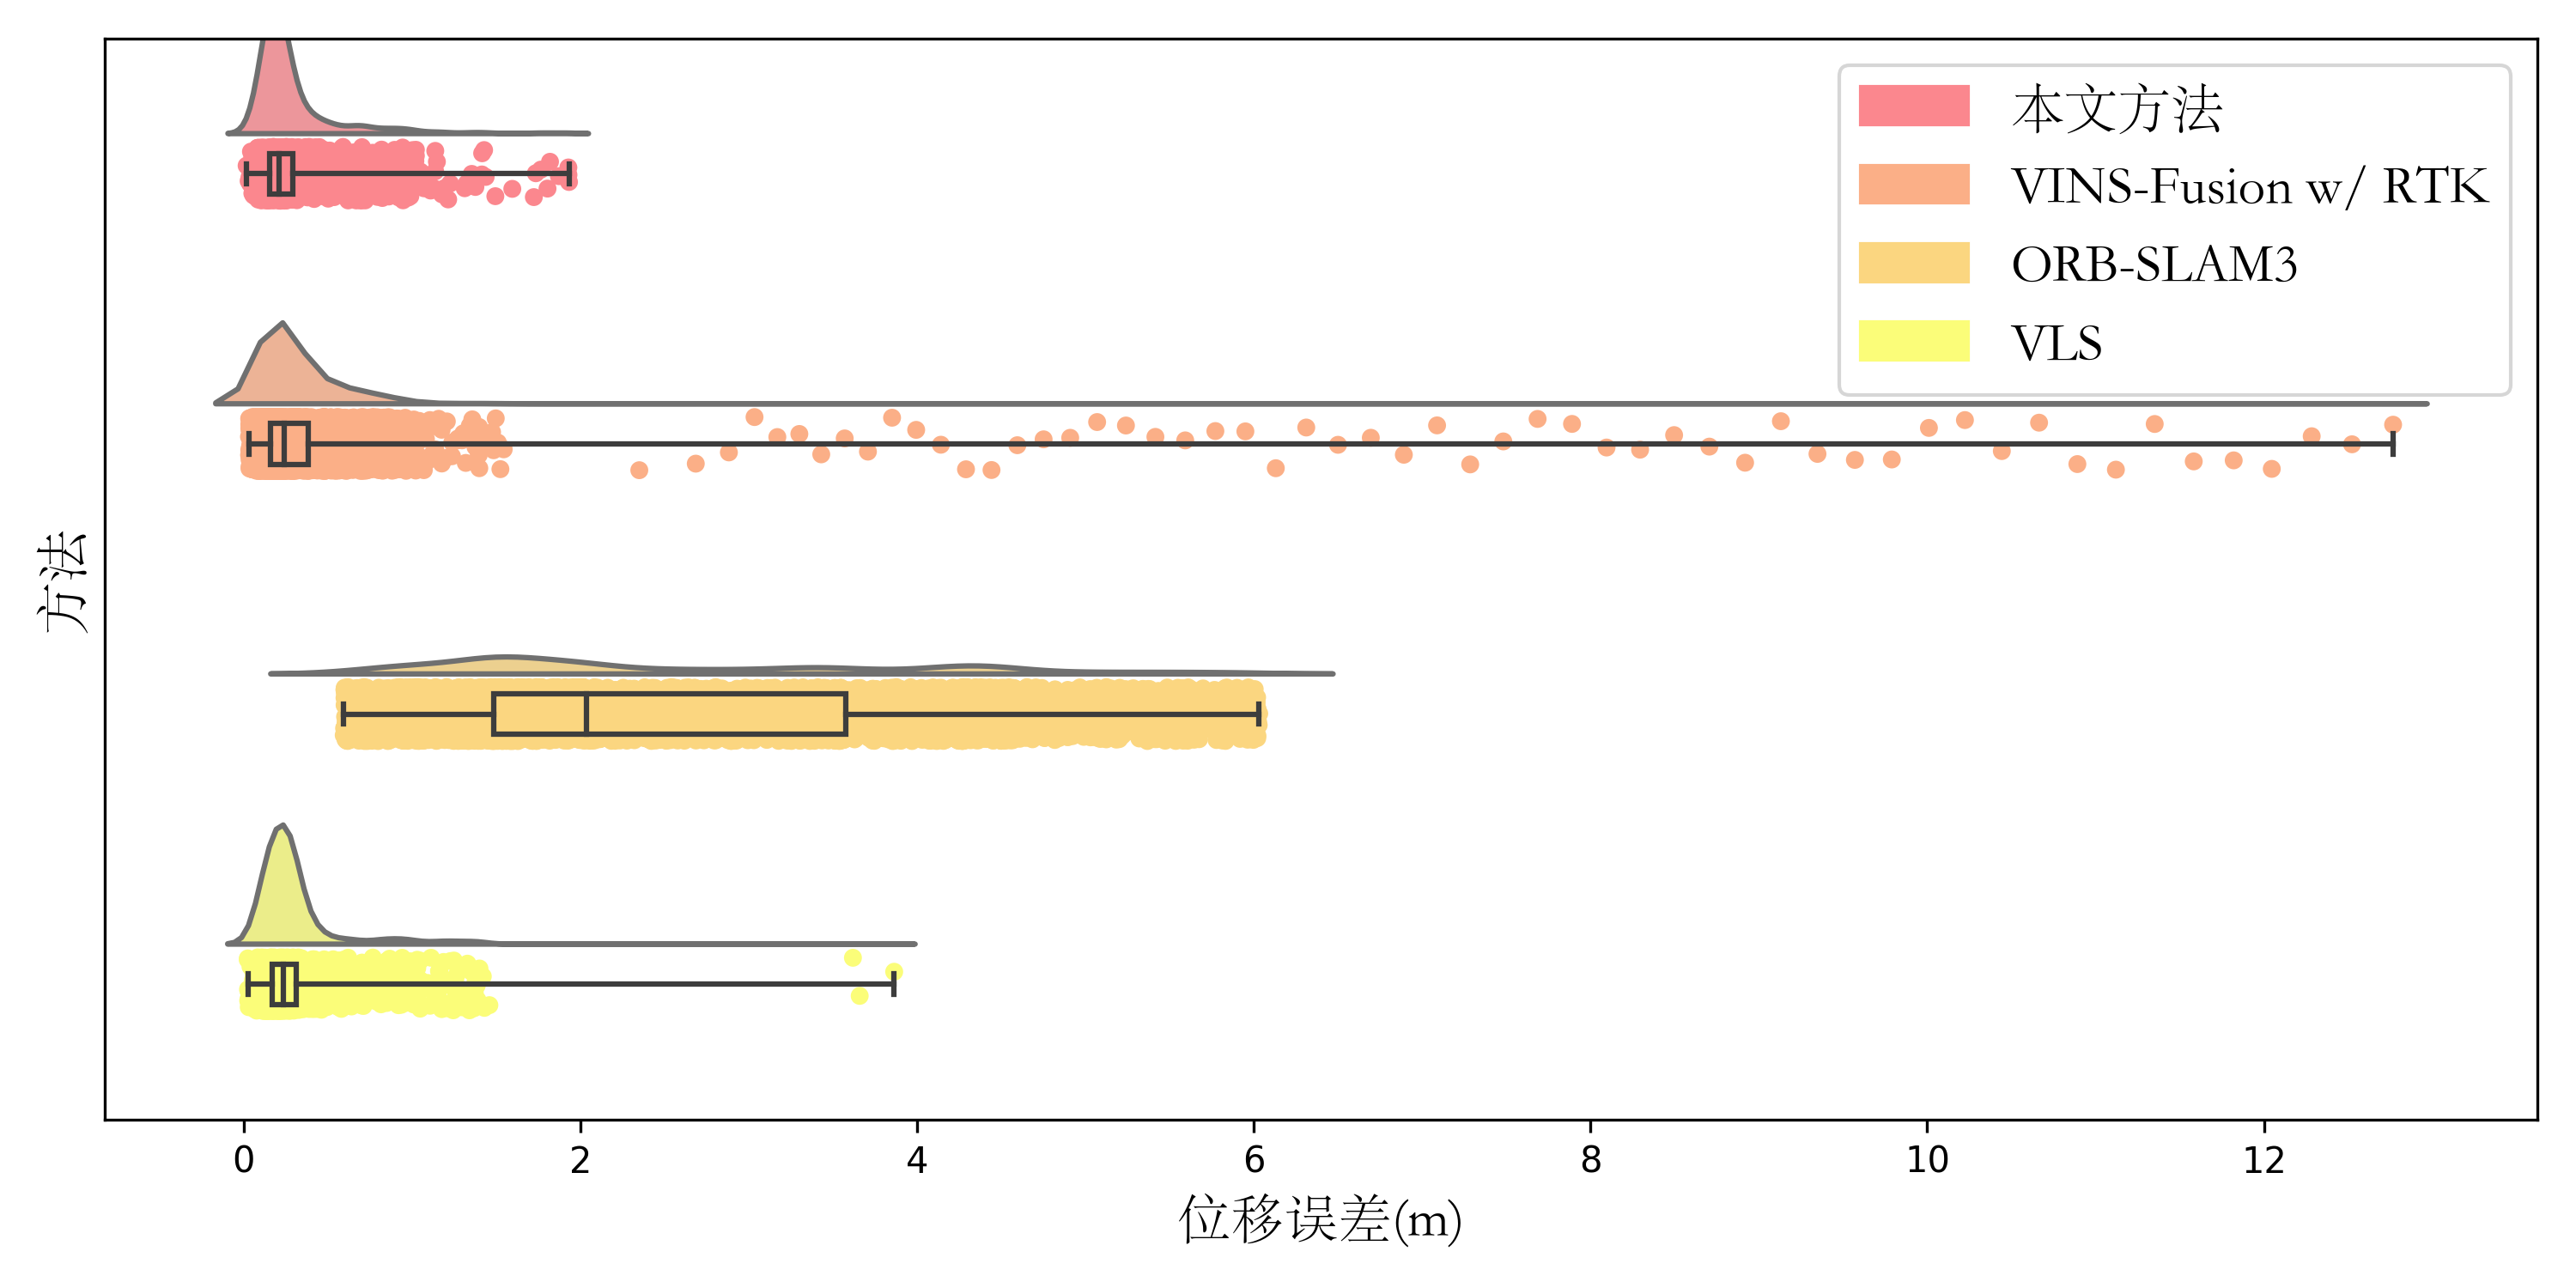
\includegraphics[width=0.8\linewidth]{loc_NH5_cloud.png}
  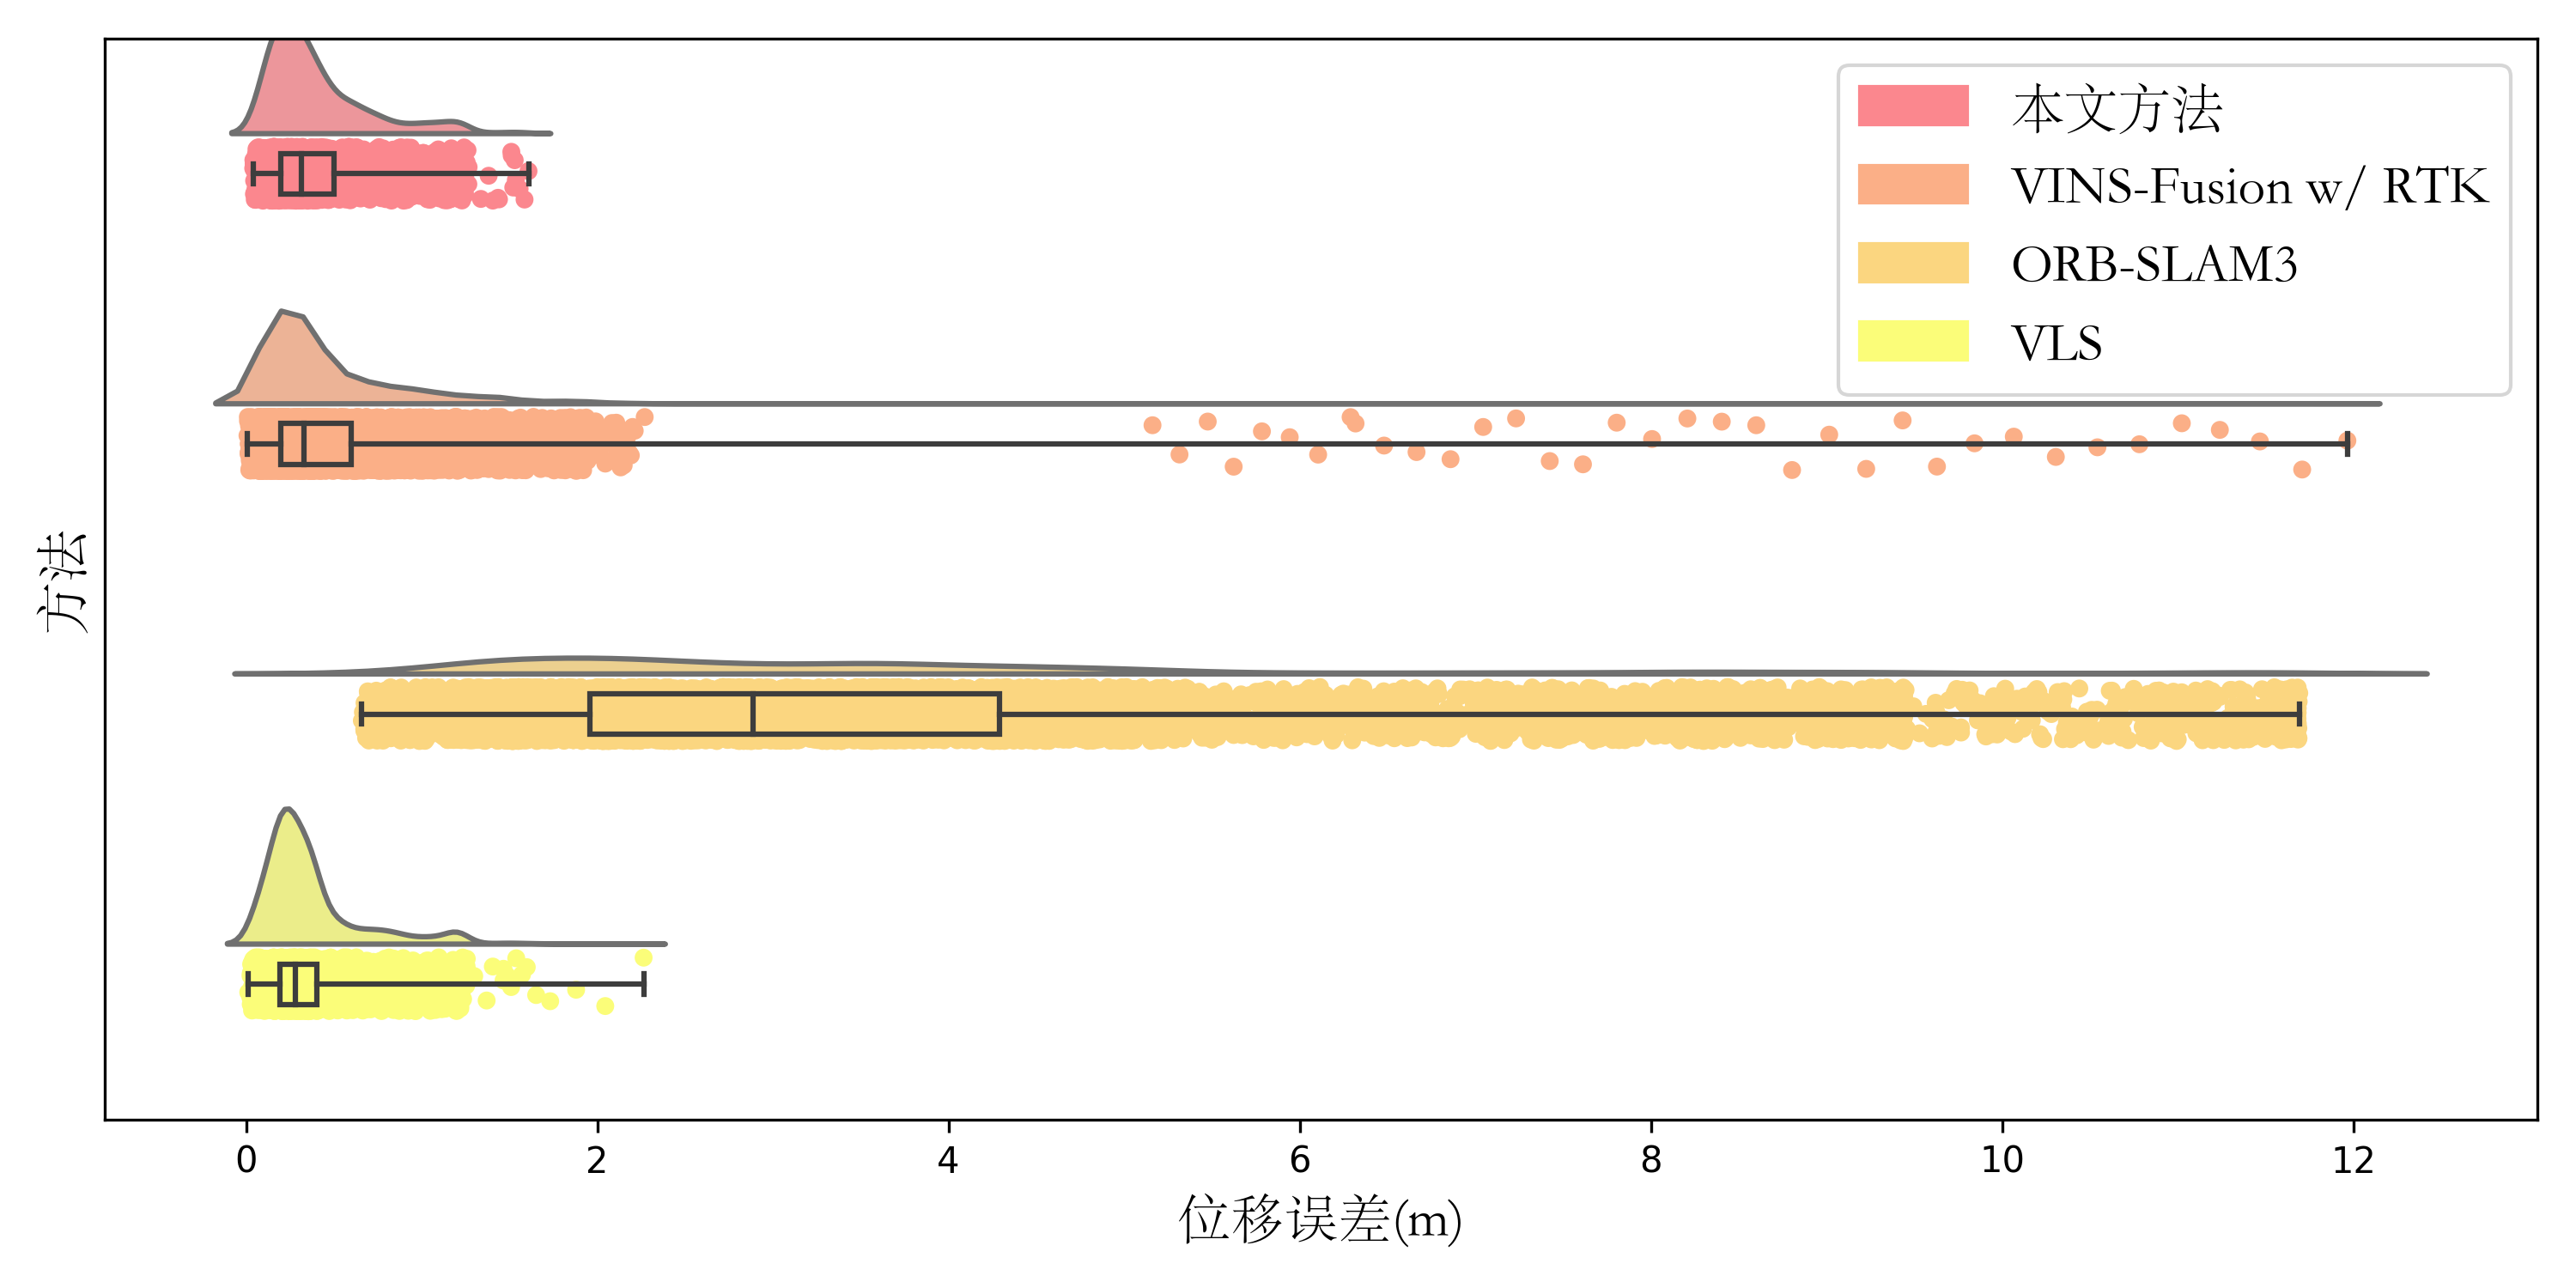
\includegraphics[width=0.8\linewidth]{loc_NH6_cloud.png}
  \caption{不同定位方法在OF5(上)和OF6(下)序列上的定位误差分布}
  \label{fig:loc_4seaons_nh5}
\end{figure}

% \begin{figure}
%   \centering
%   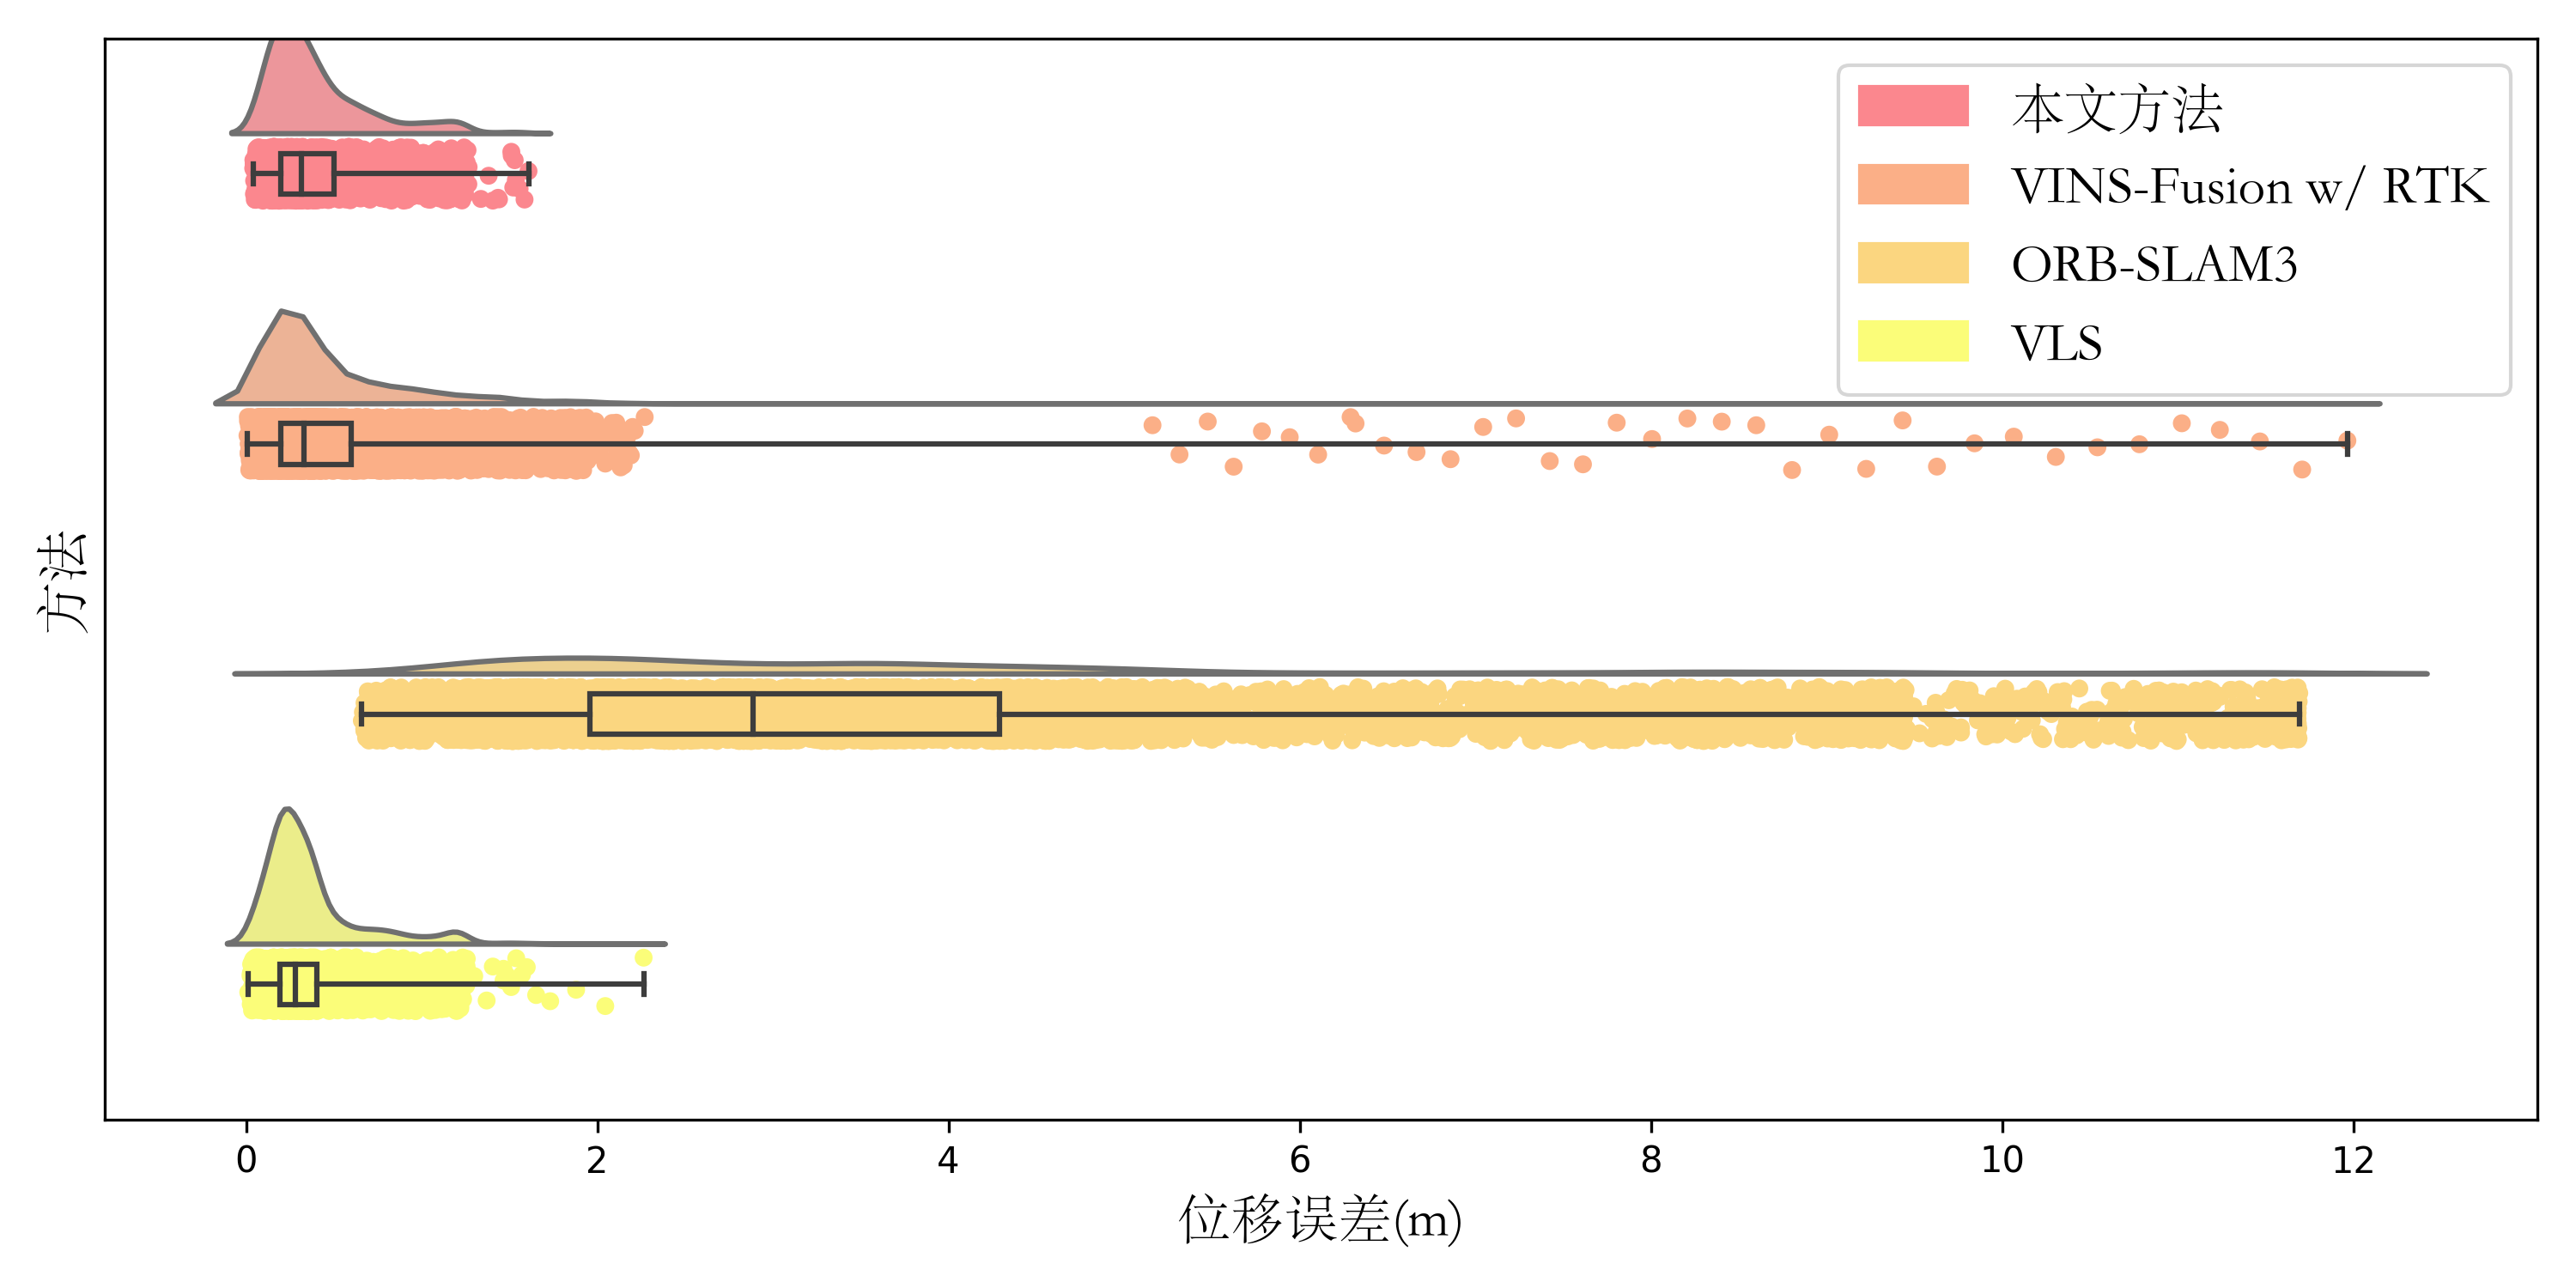
\includegraphics[width=1.0\linewidth]{loc_NH6_cloud.png}
%   \caption{不同定位方法在OF6序列上的定位误差分布}
%   \label{fig:loc_4seaons_nh6}
% \end{figure}

\subsubsection{复杂(Business Campus与Old Town)场景测试}

Business Campus场景在校园环境中,Old Town场景在城市中心区,这两个场景的有着更多的建筑物和道路,但也有着更多的移动物体和复杂的动态场景,如图~\ref{fig:scene_bc2} 和图~\ref{fig:scene_ot2} 所示,因此在这个场景下的测试能够更好地表现出本文方法在复杂环境下的表现。此外,在场景感知条件变化方面,这两个场景也覆盖了多种季节和天气条件,在Old Twon的建图序列中还有降雨天气,如图~\ref{fig:scene_ot1} 所示,也可以反映出本文方法在较差天气建图条件下的定位表现。

\begin{figure}
  \centering
  \subcaptionbox{BC2序列复杂场景\label{fig:scene_bc2}}{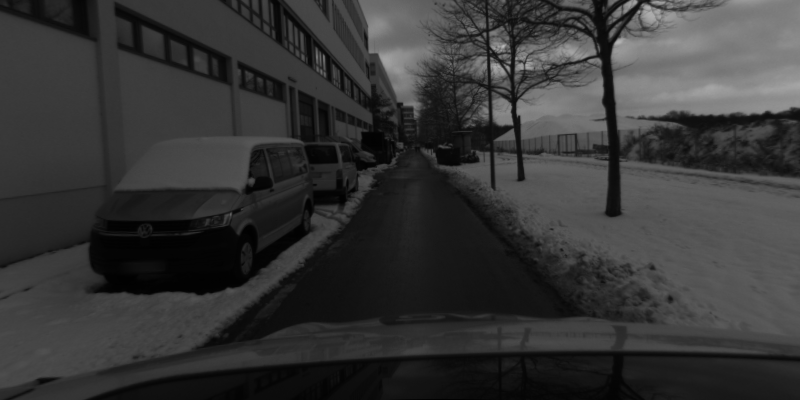
\includegraphics[width=0.32\linewidth]{BusinessCampus2.png}}
  \subcaptionbox{OT1序列降雨场景\label{fig:scene_ot1}}{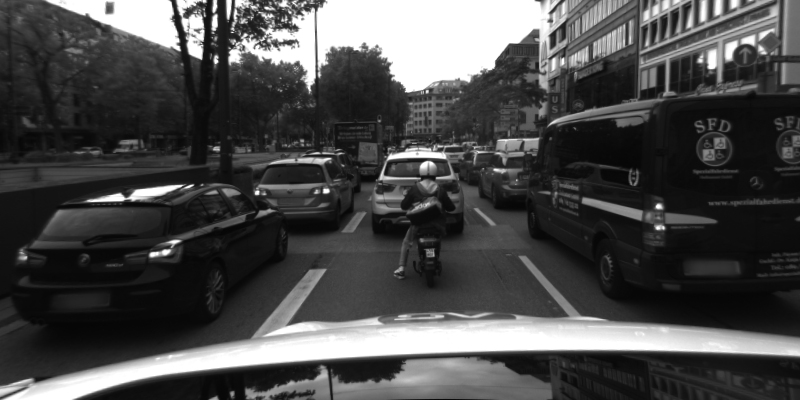
\includegraphics[width=0.32\linewidth]{OldTown1.png}}
  \subcaptionbox{OT2序列复杂场景\label{fig:scene_ot2}}{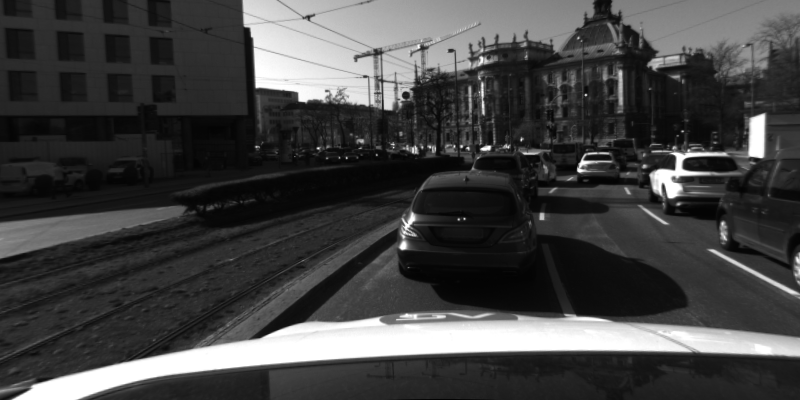
\includegraphics[width=0.32\linewidth]{OldTown2.png}}
  \caption{4Seasons数据集NH3与NH7场景差异展示}
  \label{fig:scene_bcot}
\end{figure}

在两个场景下的对比如表~\ref{tab:loc_4seaons_bc56} 和表~\ref{tab:loc_4seaons_ot2} 所示,需要注意的是,由于Business Campus场景中的建图轨迹在进行$RPE_t$和$RPE_r$指标计算的时候,对齐过程数值不稳定产生了不合理结果,因此表中只给出了建图轨迹的$ATE_t$指标,可以看到该指标非常小,足以说明建图轨迹较为精确,因此另外两个指标的缺失也是可以接受的。本文方法依旧在$ATE_t$和$RPE_t$上取得了最佳表现,但是在$RPE_r$上表现不够稳定,但是与其他方法差距非常小。此外,在这两个场景下,本文方法在定位精度上依旧取得了1米以内的误差,这不仅说明本文方法在复杂场景下的表现优秀,也说明了本文方法具有较强的稳定性。

\begin{table}
\centering
\caption{4Seasons数据集Business Campus场景部分序列指标对比}
\begin{tabular}{lccccccc}
\toprule
方法                 & 时间                                                                             & 季节                  & 天气                  & 晨昏                  & $ATE_t$\textdownarrow{}               & $RPE_t$\textdownarrow{}              & $RPE_r$\textdownarrow{}              \\ \midrule
离线建图               & \begin{tabular}[c]{@{}c@{}}10.08\\ 09:30\\ (BC1)\end{tabular}                  & 秋季                  & 晴朗                  & 清晨                  & 0.095337          & N/A               & N/A               \\ \midrule
ORB-SLAM3          & \multirow{4}{*}{\begin{tabular}[c]{@{}c@{}}01.07\\ 13:12\\ (BC2)\end{tabular}} & \multirow{4}{*}{冬季} & \multirow{4}{*}{降雪} & \multirow{4}{*}{下午} & 7.376041          & 1.668179          & \cellcolor[HTML]{FFCCC9}\textbf{1.313357} \\
VINS-Fusion w/ RTK &                                                                                &                     &                     &                     & 1.115755          & 2.313352          & 2.588801          \\
VLS                &                                                                                &                     &                     &                     & 1.092215          & 1.938506          & 1.367412 \\
本文方法               &                                                                                &                     &                     &                     & \cellcolor[HTML]{FFCCC9}\textbf{0.639282} & \cellcolor[HTML]{FFCCC9}\textbf{1.576658} & 1.385713          \\ \midrule
ORB-SLAM3          & \multirow{4}{*}{\begin{tabular}[c]{@{}c@{}}02.25\\ 14:16\\ (BC3)\end{tabular}} & \multirow{4}{*}{冬季} & \multirow{4}{*}{晴朗} & \multirow{4}{*}{下午} & 7.372700          & 1.760015          & 1.202648 \\
VINS-Fusion w/ RTK &                                                                                &                     &                     &                     & 1.076147          & 2.596570          & 2.926574          \\
VLS                &                                                                                &                     &                     &                     & 0.495447          & 2.025172          & 1.786391          \\
本文方法               &                                                                                &                     &                     &                     & \cellcolor[HTML]{FFCCC9}\textbf{0.446566} & \cellcolor[HTML]{FFCCC9}\textbf{1.380626} & \cellcolor[HTML]{FFCCC9}\textbf{1.109240}          \\ \bottomrule
\end{tabular}
\label{tab:loc_4seaons_bc56}
\end{table}

在Business Campus场景中,由于离线建图模块的精度较高,因此本文方法在定位过程中能够更好地利用地图信息,从而提升定位精度,$ATE_t$指标下都获得了50厘米左右的误差,已经有了较高的定位精度。

\begin{table}
\centering
\caption{4Seasons数据集Old Town场景第2序列指标对比}
\begin{tabular}{lccccccc}
\toprule
方法                 & 时间                                                                             & 季节                  & 天气                  & 晨昏                  & $ATE_t$\textdownarrow{}               & $RPE_t$\textdownarrow{}              & $RPE_r$\textdownarrow{}              \\ \midrule
离线建图               & \begin{tabular}[c]{@{}c@{}}10.08\\11:53\\(OT1)\end{tabular}                  & 冬季                  & 降雨                  & 清晨                  & 1.016104          & 0.456781               & 1.116236               \\ \midrule
ORB-SLAM3          & \multirow{4}{*}{\begin{tabular}[c]{@{}c@{}}02.25\\12:24\\(OT2)\end{tabular}} & \multirow{4}{*}{冬季} & \multirow{4}{*}{晴朗} & \multirow{4}{*}{清晨} & 38.930786         & 4.441040          & \cellcolor[HTML]{FFCCC9}\textbf{1.078154} \\
VINS-Fusion w/ RTK &                                                                                &                     &                     &                     & 0.965686          & 2.682027          & 1.172853          \\
VLS                &                                                                                &                     &                     &                     & 1.143163          & 2.318242          & 1.443211 \\
本文方法               &                                                                                &                     &                     &                     & \cellcolor[HTML]{FFCCC9}\textbf{0.846396} & \cellcolor[HTML]{FFCCC9}\textbf{2.318242} & 1.521039          \\ \bottomrule
\end{tabular}
\label{tab:loc_4seaons_ot2}
\end{table}

但是在Old Town场景中,由于建图序列的天气情况较差,所以轨迹的精度较低,而在这种条件下本文的定位方法依旧达到了1米以内的定位精度,这说明本文方法对于建图质量的要求并不十分苛刻,在较差的建图精度下还可以通过定位给出更加精确的结果。

\subsection{消融实验}

为了验证地图定位中的各个模块对定位精度的影响,本文进行了一系列的消融实验。在这些实验中,本文逐步增加地图定位中的各个子模块,从而验证了这些模块对定位精度的影响。具体实验结果如表~\ref{tab:loc_ablation} 所示,表中主要研究了“PO-VIO”、“粗到细定位”、“转换矩阵更新”、“相邻帧边”、“地图关键帧边”、“地图观测边”、“地图点先验边”和“真值地图”这8个变量对地图定位的影响,实验设置在Office Loop的第3条序列(OF3)上,以$ATE_t$为主要报告指标。

\begin{table}
\centering
\begin{threeparttable}
\caption{消融实验结果对比}
\begin{tabular}{ccccccccc}
\toprule
PO-VIO          & \begin{tabular}[c]{@{}c@{}}粗到细\\ 定位\end{tabular} & \begin{tabular}[c]{@{}c@{}}转换矩阵\\ 更新\end{tabular} & \begin{tabular}[c]{@{}c@{}}相邻帧\\ 边\end{tabular} & \begin{tabular}[c]{@{}c@{}}地图\\ 关键帧边\end{tabular} & \begin{tabular}[c]{@{}c@{}}地图\\ 观测边\end{tabular} & \begin{tabular}[c]{@{}c@{}}地图点\\ 先验边\end{tabular} & \begin{tabular}[c]{@{}c@{}}真值 \\ 地图 \end{tabular} & $ATE_t$    \\ \midrule
$\checkmark$ &                                                  &                                                   &                                                 &                                                   &                                                  &                                                   &                                                 & 17.193425      \\
              & $\checkmark$                                     &                                                   &                                                 &                                                   &                                                  &                                                   &                                                 & \textgreater{}60     \\
$\checkmark$ & $\checkmark$                                     &                                                  &                                                 &                                                   &                                                  &                                                   &                                                 & \underline{6.987066} \\
$\checkmark$ & $\checkmark$                                     &$\checkmark$                                                   &                                                 &                                                   &                                                  &                                                   &                                                 & 1.898881 \\
$\checkmark$ & $\checkmark$                                     &$\checkmark$                                                   & $\checkmark$                                    &                                                   &                                                  &                                                   &                                                 & 1.445279       \\
$\checkmark$ & $\checkmark$                                     &$\checkmark$                                                   & $\checkmark$                                    & $\checkmark$                                      &                                                  &                                                   &                                                 & 1.237693       \\
$\checkmark$ & $\checkmark$                                     &$\checkmark$                                                   & $\checkmark$                                    & $\checkmark$                                      & $\checkmark$                                     &                                                   &                                                 & 1.223113       \\
$\checkmark$ & $\checkmark$                                     &$\checkmark$                                                   & $\checkmark$                                    & $\checkmark$                                      & $\checkmark$                                     & $\checkmark$                                      &                                                 & 0.938238       \\
$\checkmark$ & $\checkmark$                                     &$\checkmark$                                                   & $\checkmark$                                    & $\checkmark$                                      & $\checkmark$                                     & $\checkmark$                                      & $\checkmark$                                    & 0.396039       \\ \bottomrule
\end{tabular}
\label{tab:loc_ablation}
\begin{tablenotes}
  \item [a] 实验构建在Office Loop的第3条序列(OF3)上
  \item [b] \underline{下划线}表示该序列在后期因为转换矩阵未更新而粗到细定位失败
\end{tablenotes}
\end{threeparttable}
\end{table}

在表~\ref{tab:loc_ablation} 中只有“粗到细定位”时产生了较大的定位误差,这是因为在PO-VIO和转换矩阵为粗到细定位提供先验位置信息的时候,粗到细定位的粗定位仅使用粗粒度特征产生了误匹配,从而将整个定位误差增长到了一个难以接受的程度。在第三行,当使用了VIO和转换矩阵后,这一定位误差极大得缩小到了一个可以接受的程度,这说明本文使用的转换矩阵具有非常重要的作用。但是在仅有转换矩阵而不维护的情况下,在序列的后段,由于PO-VIO的累积误差越来越大,使得转换矩阵不再能准确反映当前VIO结果和全局坐标系的正确关系,此时粗到细定位的先验位置信息也失去了意义,所以定位失败,因此表中的数据以下划线表示其是不完整序列的定位数据。在加入了转换矩阵更新之后,估计不完整的问题得到了解决,定位精度得到了进一步的提升。

在第四行到第七行中,逐步加入了相邻帧边、地图关键帧边、地图观测边和地图点先验边,可以看到这些边的加入都使得定位精度得到了进一步的提升,这说明这些边对于定位精度的提升都是有益的。这表明本文所提出的紧耦合优化中的各个残差边都是对定位结果有正向作用的。

在最后一行中,加入了真值地图,可以看到定位精度得到了进一步的提升,这说明真值地图对于定位精度的提升是有益的。在使用了真值地图后,定位精度达到了30厘米左右,这可以看作是本文方法的定位精度上限,而这也与4Seasons数据集中实验情况相符:在建图精度不足的情况下,本文方法的精度上限受到地图精度的限制(例如Office Loop场景和Old Town场景),但是在建图精度较高的情况下,本文方法的定位精度上限只由紧耦合地图定位模块的精度决定(例如Neighborhood场景和Business Campus场景)。

\subsection{系统效率测试}

\begin{table}
\centering
\caption{本文地图定位模块运行时间测试}
\begin{threeparttable}
\begin{tabular}{lccccccc}
  \toprule
  实现方法     & \begin{tabular}[c]{@{}c@{}}粗特征\\ 提取$^{\dagger}$\end{tabular} & \begin{tabular}[c]{@{}c@{}}粗特征\\ 匹配\end{tabular} & \begin{tabular}[c]{@{}c@{}}细特征\\ 提取+匹配$^{\dagger}$\end{tabular} & \begin{tabular}[c]{@{}c@{}}概率投票\\ 定位\end{tabular} & 优化                   & 其他                   & 总计    \\ \midrule
  TensorRT & 9.0                                              & \multirow{2}{*}{0.4}                             & 4.2+20.1                                            & \multirow{2}{*}{3.5}                              & \multirow{2}{*}{1.4} & \multirow{2}{*}{0.1} & 38.7  \\
  PyTorch  & 22.2                                             &                                                  & 59.8+242.6                                          &                                                   &                      &                      & 330.0 \\ \bottomrule
  \end{tabular}
\label{tab:efficiency}
\begin{tablenotes}
  \item [a] 时间单位为毫秒(ms)
  \item [b] ${\dagger}$表示此过程使用神经网络类方法
\end{tablenotes}
\end{threeparttable}
\end{table}

\section{本章总结}

本章主要以实验验证的方式对本文所提出的固定路线定位方法进行了评估。首先,本章对实验实施的平台进行了介绍,包括实验所使用的数据集、实验所使用的硬件平台和软件平台以及实验的评估指标包括绝对轨迹误差和相对姿态误差。然后本章分别针对3个模块的性能进行了测试,并与一些常规方法进行对比,分析了本文方法的优势所在以及不足之处,在重要模块中还增加了消融实验来详细验证模块内组成部分对整体精度的影响。最后,本章对实验结果进行了总结,验证了本文方法的有效性和鲁棒性。